
\documentclass{article} % For LaTeX2e
\usepackage{src/iclr2027_conference,times}

% Optional math commands from https://github.com/goodfeli/dlbook_notation.
%%%%% NEW MATH DEFINITIONS %%%%%

\usepackage{amsmath,amsfonts,bm}

% Mark sections of captions for referring to divisions of figures
\newcommand{\figleft}{{\em (Left)}}
\newcommand{\figcenter}{{\em (Center)}}
\newcommand{\figright}{{\em (Right)}}
\newcommand{\figtop}{{\em (Top)}}
\newcommand{\figbottom}{{\em (Bottom)}}
\newcommand{\captiona}{{\em (a)}}
\newcommand{\captionb}{{\em (b)}}
\newcommand{\captionc}{{\em (c)}}
\newcommand{\captiond}{{\em (d)}}

% Highlight a newly defined term
\newcommand{\newterm}[1]{{\bf #1}}


% Figure reference, lower-case.
\def\figref#1{figure~\ref{#1}}
% Figure reference, capital. For start of sentence
\def\Figref#1{Figure~\ref{#1}}
\def\twofigref#1#2{figures \ref{#1} and \ref{#2}}
\def\quadfigref#1#2#3#4{figures \ref{#1}, \ref{#2}, \ref{#3} and \ref{#4}}
% Section reference, lower-case.
\def\secref#1{section~\ref{#1}}
% Section reference, capital.
\def\Secref#1{Section~\ref{#1}}
% Reference to two sections.
\def\twosecrefs#1#2{sections \ref{#1} and \ref{#2}}
% Reference to three sections.
\def\secrefs#1#2#3{sections \ref{#1}, \ref{#2} and \ref{#3}}
% Reference to an equation, lower-case.
\def\eqref#1{equation~\ref{#1}}
% Reference to an equation, upper case
\def\Eqref#1{Equation~\ref{#1}}
% A raw reference to an equation---avoid using if possible
\def\plaineqref#1{\ref{#1}}
% Reference to a chapter, lower-case.
\def\chapref#1{chapter~\ref{#1}}
% Reference to an equation, upper case.
\def\Chapref#1{Chapter~\ref{#1}}
% Reference to a range of chapters
\def\rangechapref#1#2{chapters\ref{#1}--\ref{#2}}
% Reference to an algorithm, lower-case.
\def\algref#1{algorithm~\ref{#1}}
% Reference to an algorithm, upper case.
\def\Algref#1{Algorithm~\ref{#1}}
\def\twoalgref#1#2{algorithms \ref{#1} and \ref{#2}}
\def\Twoalgref#1#2{Algorithms \ref{#1} and \ref{#2}}
% Reference to a part, lower case
\def\partref#1{part~\ref{#1}}
% Reference to a part, upper case
\def\Partref#1{Part~\ref{#1}}
\def\twopartref#1#2{parts \ref{#1} and \ref{#2}}

\def\ceil#1{\lceil #1 \rceil}
\def\floor#1{\lfloor #1 \rfloor}
\def\1{\bm{1}}
\newcommand{\train}{\mathcal{D}}
\newcommand{\valid}{\mathcal{D_{\mathrm{valid}}}}
\newcommand{\test}{\mathcal{D_{\mathrm{test}}}}

\def\eps{{\epsilon}}


% Random variables
\def\reta{{\textnormal{$\eta$}}}
\def\ra{{\textnormal{a}}}
\def\rb{{\textnormal{b}}}
\def\rc{{\textnormal{c}}}
\def\rd{{\textnormal{d}}}
\def\re{{\textnormal{e}}}
\def\rf{{\textnormal{f}}}
\def\rg{{\textnormal{g}}}
\def\rh{{\textnormal{h}}}
\def\ri{{\textnormal{i}}}
\def\rj{{\textnormal{j}}}
\def\rk{{\textnormal{k}}}
\def\rl{{\textnormal{l}}}
% rm is already a command, just don't name any random variables m
\def\rn{{\textnormal{n}}}
\def\ro{{\textnormal{o}}}
\def\rp{{\textnormal{p}}}
\def\rq{{\textnormal{q}}}
\def\rr{{\textnormal{r}}}
\def\rs{{\textnormal{s}}}
\def\rt{{\textnormal{t}}}
\def\ru{{\textnormal{u}}}
\def\rv{{\textnormal{v}}}
\def\rw{{\textnormal{w}}}
\def\rx{{\textnormal{x}}}
\def\ry{{\textnormal{y}}}
\def\rz{{\textnormal{z}}}

% Random vectors
\def\rvepsilon{{\mathbf{\epsilon}}}
\def\rvtheta{{\mathbf{\theta}}}
\def\rva{{\mathbf{a}}}
\def\rvb{{\mathbf{b}}}
\def\rvc{{\mathbf{c}}}
\def\rvd{{\mathbf{d}}}
\def\rve{{\mathbf{e}}}
\def\rvf{{\mathbf{f}}}
\def\rvg{{\mathbf{g}}}
\def\rvh{{\mathbf{h}}}
\def\rvu{{\mathbf{i}}}
\def\rvj{{\mathbf{j}}}
\def\rvk{{\mathbf{k}}}
\def\rvl{{\mathbf{l}}}
\def\rvm{{\mathbf{m}}}
\def\rvn{{\mathbf{n}}}
\def\rvo{{\mathbf{o}}}
\def\rvp{{\mathbf{p}}}
\def\rvq{{\mathbf{q}}}
\def\rvr{{\mathbf{r}}}
\def\rvs{{\mathbf{s}}}
\def\rvt{{\mathbf{t}}}
\def\rvu{{\mathbf{u}}}
\def\rvv{{\mathbf{v}}}
\def\rvw{{\mathbf{w}}}
\def\rvx{{\mathbf{x}}}
\def\rvy{{\mathbf{y}}}
\def\rvz{{\mathbf{z}}}

% Elements of random vectors
\def\erva{{\textnormal{a}}}
\def\ervb{{\textnormal{b}}}
\def\ervc{{\textnormal{c}}}
\def\ervd{{\textnormal{d}}}
\def\erve{{\textnormal{e}}}
\def\ervf{{\textnormal{f}}}
\def\ervg{{\textnormal{g}}}
\def\ervh{{\textnormal{h}}}
\def\ervi{{\textnormal{i}}}
\def\ervj{{\textnormal{j}}}
\def\ervk{{\textnormal{k}}}
\def\ervl{{\textnormal{l}}}
\def\ervm{{\textnormal{m}}}
\def\ervn{{\textnormal{n}}}
\def\ervo{{\textnormal{o}}}
\def\ervp{{\textnormal{p}}}
\def\ervq{{\textnormal{q}}}
\def\ervr{{\textnormal{r}}}
\def\ervs{{\textnormal{s}}}
\def\ervt{{\textnormal{t}}}
\def\ervu{{\textnormal{u}}}
\def\ervv{{\textnormal{v}}}
\def\ervw{{\textnormal{w}}}
\def\ervx{{\textnormal{x}}}
\def\ervy{{\textnormal{y}}}
\def\ervz{{\textnormal{z}}}

% Random matrices
\def\rmA{{\mathbf{A}}}
\def\rmB{{\mathbf{B}}}
\def\rmC{{\mathbf{C}}}
\def\rmD{{\mathbf{D}}}
\def\rmE{{\mathbf{E}}}
\def\rmF{{\mathbf{F}}}
\def\rmG{{\mathbf{G}}}
\def\rmH{{\mathbf{H}}}
\def\rmI{{\mathbf{I}}}
\def\rmJ{{\mathbf{J}}}
\def\rmK{{\mathbf{K}}}
\def\rmL{{\mathbf{L}}}
\def\rmM{{\mathbf{M}}}
\def\rmN{{\mathbf{N}}}
\def\rmO{{\mathbf{O}}}
\def\rmP{{\mathbf{P}}}
\def\rmQ{{\mathbf{Q}}}
\def\rmR{{\mathbf{R}}}
\def\rmS{{\mathbf{S}}}
\def\rmT{{\mathbf{T}}}
\def\rmU{{\mathbf{U}}}
\def\rmV{{\mathbf{V}}}
\def\rmW{{\mathbf{W}}}
\def\rmX{{\mathbf{X}}}
\def\rmY{{\mathbf{Y}}}
\def\rmZ{{\mathbf{Z}}}

% Elements of random matrices
\def\ermA{{\textnormal{A}}}
\def\ermB{{\textnormal{B}}}
\def\ermC{{\textnormal{C}}}
\def\ermD{{\textnormal{D}}}
\def\ermE{{\textnormal{E}}}
\def\ermF{{\textnormal{F}}}
\def\ermG{{\textnormal{G}}}
\def\ermH{{\textnormal{H}}}
\def\ermI{{\textnormal{I}}}
\def\ermJ{{\textnormal{J}}}
\def\ermK{{\textnormal{K}}}
\def\ermL{{\textnormal{L}}}
\def\ermM{{\textnormal{M}}}
\def\ermN{{\textnormal{N}}}
\def\ermO{{\textnormal{O}}}
\def\ermP{{\textnormal{P}}}
\def\ermQ{{\textnormal{Q}}}
\def\ermR{{\textnormal{R}}}
\def\ermS{{\textnormal{S}}}
\def\ermT{{\textnormal{T}}}
\def\ermU{{\textnormal{U}}}
\def\ermV{{\textnormal{V}}}
\def\ermW{{\textnormal{W}}}
\def\ermX{{\textnormal{X}}}
\def\ermY{{\textnormal{Y}}}
\def\ermZ{{\textnormal{Z}}}

% Vectors
\def\vzero{{\bm{0}}}
\def\vone{{\bm{1}}}
\def\vmu{{\bm{\mu}}}
\def\vtheta{{\bm{\theta}}}
\def\va{{\bm{a}}}
\def\vb{{\bm{b}}}
\def\vc{{\bm{c}}}
\def\vd{{\bm{d}}}
\def\ve{{\bm{e}}}
\def\vf{{\bm{f}}}
\def\vg{{\bm{g}}}
\def\vh{{\bm{h}}}
\def\vi{{\bm{i}}}
\def\vj{{\bm{j}}}
\def\vk{{\bm{k}}}
\def\vl{{\bm{l}}}
\def\vm{{\bm{m}}}
\def\vn{{\bm{n}}}
\def\vo{{\bm{o}}}
\def\vp{{\bm{p}}}
\def\vq{{\bm{q}}}
\def\vr{{\bm{r}}}
\def\vs{{\bm{s}}}
\def\vt{{\bm{t}}}
\def\vu{{\bm{u}}}
\def\vv{{\bm{v}}}
\def\vw{{\bm{w}}}
\def\vx{{\bm{x}}}
\def\vy{{\bm{y}}}
\def\vz{{\bm{z}}}

% Elements of vectors
\def\evalpha{{\alpha}}
\def\evbeta{{\beta}}
\def\evepsilon{{\epsilon}}
\def\evlambda{{\lambda}}
\def\evomega{{\omega}}
\def\evmu{{\mu}}
\def\evpsi{{\psi}}
\def\evsigma{{\sigma}}
\def\evtheta{{\theta}}
\def\eva{{a}}
\def\evb{{b}}
\def\evc{{c}}
\def\evd{{d}}
\def\eve{{e}}
\def\evf{{f}}
\def\evg{{g}}
\def\evh{{h}}
\def\evi{{i}}
\def\evj{{j}}
\def\evk{{k}}
\def\evl{{l}}
\def\evm{{m}}
\def\evn{{n}}
\def\evo{{o}}
\def\evp{{p}}
\def\evq{{q}}
\def\evr{{r}}
\def\evs{{s}}
\def\evt{{t}}
\def\evu{{u}}
\def\evv{{v}}
\def\evw{{w}}
\def\evx{{x}}
\def\evy{{y}}
\def\evz{{z}}

% Matrix
\def\mA{{\bm{A}}}
\def\mB{{\bm{B}}}
\def\mC{{\bm{C}}}
\def\mD{{\bm{D}}}
\def\mE{{\bm{E}}}
\def\mF{{\bm{F}}}
\def\mG{{\bm{G}}}
\def\mH{{\bm{H}}}
\def\mI{{\bm{I}}}
\def\mJ{{\bm{J}}}
\def\mK{{\bm{K}}}
\def\mL{{\bm{L}}}
\def\mM{{\bm{M}}}
\def\mN{{\bm{N}}}
\def\mO{{\bm{O}}}
\def\mP{{\bm{P}}}
\def\mQ{{\bm{Q}}}
\def\mR{{\bm{R}}}
\def\mS{{\bm{S}}}
\def\mT{{\bm{T}}}
\def\mU{{\bm{U}}}
\def\mV{{\bm{V}}}
\def\mW{{\bm{W}}}
\def\mX{{\bm{X}}}
\def\mY{{\bm{Y}}}
\def\mZ{{\bm{Z}}}
\def\mBeta{{\bm{\beta}}}
\def\mPhi{{\bm{\Phi}}}
\def\mLambda{{\bm{\Lambda}}}
\def\mSigma{{\bm{\Sigma}}}

% Tensor
\DeclareMathAlphabet{\mathsfit}{\encodingdefault}{\sfdefault}{m}{sl}
\SetMathAlphabet{\mathsfit}{bold}{\encodingdefault}{\sfdefault}{bx}{n}
\newcommand{\tens}[1]{\bm{\mathsfit{#1}}}
\def\tA{{\tens{A}}}
\def\tB{{\tens{B}}}
\def\tC{{\tens{C}}}
\def\tD{{\tens{D}}}
\def\tE{{\tens{E}}}
\def\tF{{\tens{F}}}
\def\tG{{\tens{G}}}
\def\tH{{\tens{H}}}
\def\tI{{\tens{I}}}
\def\tJ{{\tens{J}}}
\def\tK{{\tens{K}}}
\def\tL{{\tens{L}}}
\def\tM{{\tens{M}}}
\def\tN{{\tens{N}}}
\def\tO{{\tens{O}}}
\def\tP{{\tens{P}}}
\def\tQ{{\tens{Q}}}
\def\tR{{\tens{R}}}
\def\tS{{\tens{S}}}
\def\tT{{\tens{T}}}
\def\tU{{\tens{U}}}
\def\tV{{\tens{V}}}
\def\tW{{\tens{W}}}
\def\tX{{\tens{X}}}
\def\tY{{\tens{Y}}}
\def\tZ{{\tens{Z}}}


% Graph
\def\gA{{\mathcal{A}}}
\def\gB{{\mathcal{B}}}
\def\gC{{\mathcal{C}}}
\def\gD{{\mathcal{D}}}
\def\gE{{\mathcal{E}}}
\def\gF{{\mathcal{F}}}
\def\gG{{\mathcal{G}}}
\def\gH{{\mathcal{H}}}
\def\gI{{\mathcal{I}}}
\def\gJ{{\mathcal{J}}}
\def\gK{{\mathcal{K}}}
\def\gL{{\mathcal{L}}}
\def\gM{{\mathcal{M}}}
\def\gN{{\mathcal{N}}}
\def\gO{{\mathcal{O}}}
\def\gP{{\mathcal{P}}}
\def\gQ{{\mathcal{Q}}}
\def\gR{{\mathcal{R}}}
\def\gS{{\mathcal{S}}}
\def\gT{{\mathcal{T}}}
\def\gU{{\mathcal{U}}}
\def\gV{{\mathcal{V}}}
\def\gW{{\mathcal{W}}}
\def\gX{{\mathcal{X}}}
\def\gY{{\mathcal{Y}}}
\def\gZ{{\mathcal{Z}}}

% Sets
\def\sA{{\mathbb{A}}}
\def\sB{{\mathbb{B}}}
\def\sC{{\mathbb{C}}}
\def\sD{{\mathbb{D}}}
% Don't use a set called E, because this would be the same as our symbol
% for expectation.
\def\sF{{\mathbb{F}}}
\def\sG{{\mathbb{G}}}
\def\sH{{\mathbb{H}}}
\def\sI{{\mathbb{I}}}
\def\sJ{{\mathbb{J}}}
\def\sK{{\mathbb{K}}}
\def\sL{{\mathbb{L}}}
\def\sM{{\mathbb{M}}}
\def\sN{{\mathbb{N}}}
\def\sO{{\mathbb{O}}}
\def\sP{{\mathbb{P}}}
\def\sQ{{\mathbb{Q}}}
\def\sR{{\mathbb{R}}}
\def\sS{{\mathbb{S}}}
\def\sT{{\mathbb{T}}}
\def\sU{{\mathbb{U}}}
\def\sV{{\mathbb{V}}}
\def\sW{{\mathbb{W}}}
\def\sX{{\mathbb{X}}}
\def\sY{{\mathbb{Y}}}
\def\sZ{{\mathbb{Z}}}

% Entries of a matrix
\def\emLambda{{\Lambda}}
\def\emA{{A}}
\def\emB{{B}}
\def\emC{{C}}
\def\emD{{D}}
\def\emE{{E}}
\def\emF{{F}}
\def\emG{{G}}
\def\emH{{H}}
\def\emI{{I}}
\def\emJ{{J}}
\def\emK{{K}}
\def\emL{{L}}
\def\emM{{M}}
\def\emN{{N}}
\def\emO{{O}}
\def\emP{{P}}
\def\emQ{{Q}}
\def\emR{{R}}
\def\emS{{S}}
\def\emT{{T}}
\def\emU{{U}}
\def\emV{{V}}
\def\emW{{W}}
\def\emX{{X}}
\def\emY{{Y}}
\def\emZ{{Z}}
\def\emSigma{{\Sigma}}

% entries of a tensor
% Same font as tensor, without \bm wrapper
\newcommand{\etens}[1]{\mathsfit{#1}}
\def\etLambda{{\etens{\Lambda}}}
\def\etA{{\etens{A}}}
\def\etB{{\etens{B}}}
\def\etC{{\etens{C}}}
\def\etD{{\etens{D}}}
\def\etE{{\etens{E}}}
\def\etF{{\etens{F}}}
\def\etG{{\etens{G}}}
\def\etH{{\etens{H}}}
\def\etI{{\etens{I}}}
\def\etJ{{\etens{J}}}
\def\etK{{\etens{K}}}
\def\etL{{\etens{L}}}
\def\etM{{\etens{M}}}
\def\etN{{\etens{N}}}
\def\etO{{\etens{O}}}
\def\etP{{\etens{P}}}
\def\etQ{{\etens{Q}}}
\def\etR{{\etens{R}}}
\def\etS{{\etens{S}}}
\def\etT{{\etens{T}}}
\def\etU{{\etens{U}}}
\def\etV{{\etens{V}}}
\def\etW{{\etens{W}}}
\def\etX{{\etens{X}}}
\def\etY{{\etens{Y}}}
\def\etZ{{\etens{Z}}}

% The true underlying data generating distribution
\newcommand{\pdata}{p_{\rm{data}}}
% The empirical distribution defined by the training set
\newcommand{\ptrain}{\hat{p}_{\rm{data}}}
\newcommand{\Ptrain}{\hat{P}_{\rm{data}}}
% The model distribution
\newcommand{\pmodel}{p_{\rm{model}}}
\newcommand{\Pmodel}{P_{\rm{model}}}
\newcommand{\ptildemodel}{\tilde{p}_{\rm{model}}}
% Stochastic autoencoder distributions
\newcommand{\pencode}{p_{\rm{encoder}}}
\newcommand{\pdecode}{p_{\rm{decoder}}}
\newcommand{\precons}{p_{\rm{reconstruct}}}

\newcommand{\laplace}{\mathrm{Laplace}} % Laplace distribution

\newcommand{\E}{\mathbb{E}}
\newcommand{\Ls}{\mathcal{L}}
\newcommand{\R}{\mathbb{R}}
\newcommand{\emp}{\tilde{p}}
\newcommand{\lr}{\alpha}
\newcommand{\reg}{\lambda}
\newcommand{\rect}{\mathrm{rectifier}}
\newcommand{\softmax}{\mathrm{softmax}}
\newcommand{\sigmoid}{\sigma}
\newcommand{\softplus}{\zeta}
\newcommand{\KL}{D_{\mathrm{KL}}}
\newcommand{\Var}{\mathrm{Var}}
\newcommand{\standarderror}{\mathrm{SE}}
\newcommand{\Cov}{\mathrm{Cov}}
% Wolfram Mathworld says $L^2$ is for function spaces and $\ell^2$ is for vectors
% But then they seem to use $L^2$ for vectors throughout the site, and so does
% wikipedia.
\newcommand{\normlzero}{L^0}
\newcommand{\normlone}{L^1}
\newcommand{\normltwo}{L^2}
\newcommand{\normlp}{L^p}
\newcommand{\normmax}{L^\infty}

\newcommand{\parents}{Pa} % See usage in notation.tex. Chosen to match Daphne's book.

\DeclareMathOperator*{\argmax}{arg\,max}
\DeclareMathOperator*{\argmin}{arg\,min}

\DeclareMathOperator{\sign}{sign}
\DeclareMathOperator{\Tr}{Tr}
\let\ab\allowbreak


\usepackage{hyperref}
\usepackage{url}
\usepackage{todonotes}
\usepackage{tikz}
\usepackage{booktabs}
\usepackage{longtable}

% caption setup
\usepackage{caption}
\usetikzlibrary{positioning,arrows.meta,calc,decorations.pathreplacing}
\captionsetup{
    font=small,
    labelfont=bf
}
\newcommand{\todofig}[2][]{\todo[color=blue!15,#1]{#2}}

\title{The Behavioral Rate of Fine-Tuning:
Compression as a Measure of Useful Information}
% Compression Reveals the Structure of Learned Behavior in Language Models?


% Authors must not appear in the submitted version. They should be hidden
% as long as the \iclrfinalcopy macro remains commented out below.
% Non-anonymous submissions will be rejected without review.

\author{Joey David$^{1}$, Paul Caillon$^{1}$, Alexandre Allauzen$^{1,2}$ \\
$^1$ Miles Team, LAMSADE, Université Paris Dauphine-PSL, Paris, France \\
$^2$ ESPCI PSL, Paris, France \\
\texttt{\{name\}.\{surname\}@dauphine.psl.eu}
}

% The \author macro works with any number of authors. There are two commands
% used to separate the names and addresses of multiple authors: \And and \AND.
%
% Using \And between authors leaves it to \LaTeX{} to determine where to break
% the lines. Using \AND forces a linebreak at that point. So, if \LaTeX{}
% puts 3 of 4 authors names on the first line, and the last on the second
% line, try using \AND instead of \And before the third author name.

\newcommand{\fix}{\marginpar{FIX}}
\newcommand{\new}{\marginpar{NEW}}

%\iclrfinalcopy % Uncomment for camera-ready version, but NOT for submission.
\begin{document}
\raggedbottom

\maketitle

\begin{abstract}
Low-Rank Adaptation (LoRA) adapts a frozen language model through a compact learned update, making it a natural setting for asking how much information fine-tuning actually needs to write.
Yet adapter rank, parameter count, or numerical reconstruction error do not directly tell us how many bits are required to preserve the behavior acquired during training.
We therefore define an operational behavioral rate $R^\star$ as the exact serialized size of a compressed adapter.
It is the smallest number of bits that, once reloaded into the frozen base model, retains a fixed fraction of the adapter's held-out fine-tuning gain.
Across a broad set of LoRA fine-tuning experiments, we find that this rate increases with distinct training content at fixed optimization budgets, but is not determined by source description length, fine-tuning gain, or ordinary weight-space reconstruction error.
Most importantly, the same datasets exhibit substantially different, and even reordered, rates across frozen base models, showing that fine-tuning compressibility is a property of the dataset–receiver pair rather than of the dataset alone.
Correction spectra measured on the data rank these rates within a receiver but fail on new receivers; the best cross-receiver predictor we found reads the trained adapter's leading singular direction.
Compression can also do more than preserve behavior. Adapters trained on deliberately corrupted reasoning fall far below the frozen model; compressed, they score above it (GSM8K 23.7\% to 82.9\%, against 77.6\% for the frozen Qwen2.5-7B), in three model families and at sizes from 0.5B to 32B. The damage sits in the update's leading singular directions, and compression works mostly by shrinking them. Away from its task, the compressed corrupted adapter keeps the frozen model's accuracy where a clean fine-tune does not: on harder math it keeps 97\% of base accuracy, the clean adapter 44\%.
Together, these results suggest that the information cost of fine-tuning is not intrinsic to the data or to parameter displacement, but depends on the receiver, the target behavior, and how the required corrections are represented in the learned update.
\end{abstract}

\section{Introduction}

Transformer-based Large Language Models (LLMs) are exceptionally efficient containers of information, but remain infamously opaque to classical modular decomposition. Although modern LLMs are often described as over-parameterized, the number of bits they use to represent their parameters is small compared to the information content of their training datasets; even more so under quantization/reduced-precision frameworks. Standard language-model training minimizes prediction loss over the contents of a dataset. In this sense, learning can be viewed as a form of lossy information transfer, shaping LLMs into the most efficient compressed representations of their training corpora with respect to their training objective.
\newline
This heavily bit-constrained regime also makes tracing the writing of new information into a model, via training, fundamentally nontrivial. Even parameter-efficient post-training methods such as Low-Rank Adaptation (LoRA) \citep{hu2022lora}, despite being modular in parameter space, still induce behavioral changes through distributed interactions with the frozen model’s internal representations. When finetuning pretrained models, parameter-efficient adapters provide a clean setting for studying this process, as they isolate the written information to a parameterized update whose effective bit budget can be directly controlled.
\newline
In this work, we adopt an information-theoretic view of finetuning. We treat the task-relevant information supplied by the finetuning data as a source, and the finetuning process as an encoder of this information. The adapter in which this information is written can be thought of as a finite-rate message; as it carries a lossy parameter-space encoding of the finetuned behavior. During inference, the composition of the frozen base model and the adapter produces the acquired behavior, i.e., the reconstruction of the information supplied during training.
% --- Palette: figures4papers (paper/plots/style.py), same meanings as the plots:
% blue = the adapter / message, gray = frozen base, red = damage/distortion.
\definecolor{srcFill}{HTML}{EEF7EE}
\definecolor{srcDraw}{HTML}{8BCF8B}
\definecolor{srcIcon}{HTML}{3F8F3F}
\definecolor{encFill}{HTML}{F5EAF3}
\definecolor{encDraw}{HTML}{C28FB9}
\definecolor{encIcon}{HTML}{9A4D8E}
\definecolor{msgFill}{HTML}{E6EEF7}
\definecolor{msgDraw}{HTML}{3775BA}
\definecolor{msgIcon}{HTML}{0F4D92}
\definecolor{baseFill}{HTML}{F2F2F2}
\definecolor{decDraw}{HTML}{4D4D4D}
\definecolor{baseIcon}{HTML}{767676}
\definecolor{adpFill}{HTML}{E6EEF7}
\definecolor{adpIcon}{HTML}{0F4D92}
\definecolor{outFill}{HTML}{E5F2F3}
\definecolor{outDraw}{HTML}{42949E}
\definecolor{outIcon}{HTML}{2C6F77}
\definecolor{distDraw}{HTML}{B64342}

\begin{figure}[t]
\centering
\resizebox{\linewidth}{!}{%
\begin{tikzpicture}[
  font=\normalsize,
  >={Latex[length=2.7mm,width=2.0mm]},
  flow/.style={->,line width=1.15pt,draw=decDraw},
  panel/.style={
    rounded corners=2.5pt,
    line width=1.0pt,
    minimum width=3.15cm,
    minimum height=2.85cm,
    inner sep=0pt
  },
  role/.style={font=\bfseries\large},
  main/.style={font=\large,align=center,text=black!92},
  sub/.style={font=\itshape\normalsize}
]

% --- Main panels ---------------------------------------------------
\node[panel,draw=srcDraw,fill=srcFill] (data) at (0,0) {};
\node[panel,draw=encDraw,fill=encFill] (training) at (4.05,0) {};
\node[panel,draw=msgDraw,fill=msgFill] (adapter) at (8.10,0) {};
\node[minimum width=4.80cm,minimum height=2.85cm,inner sep=0pt] (decoder) at (13.10,0) {};
\node[panel,draw=outDraw,fill=outFill] (behavior) at (18.15,0) {};

% --- SOURCE icon: clean stacked documents --------------------------
\begin{scope}[
    shift={($(data.center)+(0,0.64)$)},
    draw=srcIcon,
    line width=1.15pt,
    scale=1.18
]

% back sheet
\draw[
    fill=srcFill,
    rounded corners=1.2pt
]
(-0.02,-0.28) rectangle (0.34,0.30);

% middle sheet
\draw[
    fill=srcFill,
    rounded corners=1.2pt
]
(-0.12,-0.20) rectangle (0.24,0.38);

% front sheet
\draw[
    fill=srcFill,
    rounded corners=1.2pt
]
(-0.22,-0.12) rectangle (0.14,0.46);

% text lines on front sheet only
\draw[line width=.9pt] (-0.14,0.26) -- (0.06,0.26);
\draw[line width=.9pt] (-0.14,0.13) -- (0.06,0.13);
\draw[line width=.9pt] (-0.14,0.00) -- (0.02,0.00);

\end{scope}
\node[main] at ($(data.center)+(0,-0.70)$) {Fine-tuning\\data};

% --- ENCODER icon --------------------------------------------------
\begin{scope}[shift={($(training.center)+(0,0.66)$)},scale=1.18]
  \foreach \a in {0,45,...,315}{\begin{scope}[rotate=\a]\fill[encIcon] (-0.08,0.29) rectangle (0.08,0.43);\end{scope}}
  \fill[encIcon] (0,0) circle (0.34);
  \fill[encFill] (0,0) circle (0.13);
\end{scope}
\node[main] at ($(training.center)+(0,-0.62)$) {Fine-tuning};

% --- MESSAGE adapter glyph ----------------------------------------
\begin{scope}[shift={($(adapter.center)+(0,0.66)$)},draw=msgIcon,line width=1.25pt,scale=1.18]
  \draw[fill=msgFill,rounded corners=2.6pt] (-0.34,-0.31) rectangle (0.40,0.31);
  \foreach \yy in {-0.18,0,0.18}{\draw (-0.50,\yy)--(-0.34,\yy);}
  \draw (0.02,-0.17)--(0.02,0.17);
  \draw (0.14,-0.17)--(0.14,0.17);
  \draw (0.26,-0.17)--(0.26,0.17);
\end{scope}
\node[main] at ($(adapter.center)+(0,-0.70)$) {Learned\\adapter};

% --- DECODER -------------------------------------------------------
\begin{scope}
  \clip[rounded corners=2.5pt] (decoder.south west) rectangle (decoder.north east);
  \fill[baseFill] (decoder.south west) rectangle (decoder.center |- decoder.north);
  \fill[adpFill] (decoder.center |- decoder.south) rectangle (decoder.north east);
\end{scope}
\draw[draw=decDraw,line width=1.0pt,rounded corners=2.5pt]
  (decoder.south west) rectangle (decoder.north east);

% docking divider
\draw[dashed,dash pattern=on 3pt off 2.4pt,draw=black!34,line width=.72pt]
  ($(decoder.center)+(0,1.425)$)--($(decoder.center)+(0,0.38)$);
\draw[draw=black!34,line width=.72pt]
  ($(decoder.center)+(0,0.38)$) arc[start angle=90,end angle=-90,radius=.20cm];
\draw[dashed,dash pattern=on 3pt off 2.4pt,draw=black!34,line width=.72pt]
  ($(decoder.center)+(0,-0.38)$)--($(decoder.center)+(0,-1.425)$);

% base-model network icon
% --- Base-model icon: compact layered neural network ----------------
\begin{scope}[
    shift={($(decoder.west)!0.5!(decoder.center)+(0,0.49)$)},
    x=0.34cm,
    y=0.27cm
]

% connections: input -> hidden
\foreach \yi in {-1,0,1}{
    \foreach \yh in {-1.35,-0.45,0.45,1.35}{
        \draw[
            draw=baseIcon!55,
            line width=0.45pt
        ] (-1,\yi) -- (0,\yh);
    }
}

% connections: hidden -> output
\foreach \yh in {-1.35,-0.45,0.45,1.35}{
    \foreach \yo in {-1,0,1}{
        \draw[
            draw=baseIcon!55,
            line width=0.45pt
        ] (0,\yh) -- (1,\yo);
    }
}

% nodes
\foreach \y in {-1,0,1}{
    \filldraw[
        fill=baseFill,
        draw=baseIcon,
        line width=0.75pt
    ] (-1,\y) circle (0.105cm);

    \filldraw[
        fill=baseFill,
        draw=baseIcon,
        line width=0.75pt
    ] (1,\y) circle (0.105cm);
}

\foreach \y in {-1.35,-0.45,0.45,1.35}{
    \filldraw[
        fill=baseFill,
        draw=baseIcon,
        line width=0.75pt
    ] (0,\y) circle (0.105cm);
}

\end{scope}
\node[font=\large,text=black!92] at ($(decoder.west)!0.5!(decoder.center)+(0,-0.48)$) {Base model};
\node[sub,text=baseIcon] at ($(decoder.west)!0.5!(decoder.center)+(0,-0.91)$) {frozen};

% matching trained-adapter glyph
\begin{scope}[shift={($(decoder.center)!0.5!(decoder.east)+(0,0.70)$)},draw=adpIcon,line width=1.25pt,scale=1.18]
  \draw[fill=adpFill,rounded corners=2.6pt] (-0.34,-0.31) rectangle (0.40,0.31);
  \foreach \yy in {-0.18,0,0.18}{\draw (-0.50,\yy)--(-0.34,\yy);}
  \draw (0.02,-0.17)--(0.02,0.17);
  \draw (0.14,-0.17)--(0.14,0.17);
  \draw (0.26,-0.17)--(0.26,0.17);
\end{scope}
\node[font=\large,text=black!92] at ($(decoder.center)!0.5!(decoder.east)+(0,-0.48)$) {Adapter};
\node[sub,text=adpIcon] at ($(decoder.center)!0.5!(decoder.east)+(0,-0.91)$) {trained};

% --- RECONSTRUCTION icon ------------------------------------------
\begin{scope}[shift={($(behavior.center)+(0,0.66)$)},draw=outIcon,line width=1.25pt,scale=1.18]
  \draw (0,0) circle (.34);
  \draw (0,0) circle (.21);
  \draw (0,0) circle (.07);
  \draw[->] (.39,.39)--(.0,.0);
\end{scope}
\node[main] at ($(behavior.center)+(0,-0.70)$) {Adapted\\behavior};

% --- Stage headings ------------------------------------------------
\node[role,text=srcIcon] at ($(data.north)+(0,1.00)$) {SOURCE};
\node[role,text=encIcon] at ($(training.north)+(0,1.00)$) {ENCODER};
\node[role,text=msgIcon] at ($(adapter.north)+(0,1.00)$) {MESSAGE};
\node[role,text=decDraw] at ($(decoder.north)+(0,1.00)$) {DECODER};
\node[role,text=outIcon] at ($(behavior.north)+(0,1.00)$) {RECONSTRUCTION};

% heading brackets
\foreach \node/\col in {data/srcIcon,training/encIcon,adapter/msgIcon,decoder/decDraw,behavior/outIcon}{
  \draw[\col,line width=.75pt,rounded corners=2pt]
    ($ (\node.north west)+(0,0.38) $)
    -- ($ (\node.north west)+(0,0.50) $)
    -- ($ (\node.north east)+(0,0.50) $)
    -- ($ (\node.north east)+(0,0.38) $);
}

% --- Main flow -----------------------------------------------------
\draw[flow] (data.east)--(training.west);
\draw[flow] (training.east)--(adapter.west);
\draw[flow] (adapter.east)--(decoder.west);
\draw[flow] (decoder.east)--(behavior.west);

% --- Rate brace ----------------------------------------------------
\draw[decorate,decoration={brace,mirror,amplitude=4.4pt},draw=msgIcon,line width=.8pt]
  ($(adapter.south west)+(0,-.12)$)--($(adapter.south east)+(0,-.12)$);
\node[font=\large,text=msgIcon] (rate) at ($(adapter.south)+(0,-.62)$) {rate $R$};

% --- Behavioral distortion ----------------------------------------
\coordinate (dbot) at ($(adapter.south)+(0,-1.46)$);
\draw[->,dash pattern=on 4pt off 3pt,line width=.9pt,draw=distDraw]
  (data.south)
  -- (data.south |- dbot)
  -- node[pos=.53,below=5pt,font=\large,text=distDraw,fill=white,inner xsep=2pt]
     {behavioral distortion $D$}
  (behavior.south |- dbot)
  -- (behavior.south);

\end{tikzpicture}%
}

\caption{Information-theoretic view of parameter-efficient fine-tuning. $R$ is the number of bits used by the adapter, $D$ measures failure to preserve the behavior induced by fine-tuning.}
\label{fig:information_view}
\end{figure}

Under this analogy, illustrated in Figure \ \ref{fig:information_view}, we can also reuse the concepts of rate $R$, as the number of bits used to represent the adapter; while distortion $D$ is a measure of the degradation of the original behavior upon reconstruction. Put together, we establish a rate-distortion relation as the trade-off between the bit budget of the adapter and the preservation of the behavior induced by finetuning. Finally, for a fixed distortion tolerance $D^\star$, we can define the behavioral rate $R^\star$ as the smallest bit budget allowing for the reconstruction of an adapter whose behavior satisfies $D^\star$. In practice, we instantiate $R$ by training an adapter once, compressing it and measuring the resulting file size, then evaluate its performance after decoding back into the frozen model. This way, we can measure $D$ behaviorally, rather than using parameter-space proxies such as the adapter's weight reconstruction error. $R^\star(D^\star)$ is thus a measure of the smallest tested file size, and can be measured in compressed adapter file bits per initial parameter.
\newline
We first show that ordinary proxies do not predict $R^\star$: neither rank, parameter count, weight reconstruction error, update magnitude nor the size of the behavioral gain sets it, and rank and precision are not interchangeable ways of spending bits. The rate is receiver-relative: the same datasets need different rates on different frozen models, sometimes in reversed order. Correction spectra measured on the data explain these differences within a receiver but not across receivers; the trained adapter's own spectrum does better.
\newline
Most importantly, we find that the information written by fine-tuning has an uneven impact. In structured tasks like reasoning-based problem-solving, training an adapter deliberately on corrupted datasets can severely damage task performance over a base model. However, by compressing the adapter, we are consistently able to recover most of the lost behavior, and even surpass the frozen base model across several types of tasks, model sizes and family. The damage sits in the adapter's leading singular directions: coarse coding works mostly by shrinking them, and removing them at full precision works as well. The compressed adapter also keeps the frozen model's accuracy on unrelated tasks, where a clean fine-tune loses it.
\newline
Together, these results suggest that finetuning information is structured into components of sharply different behavioral value, and that this value depends on both the receiver and the adapter carrier.

% svd results on corrrupted work.
\section{Related Work}

% PEFT and adapter structure
Parameter-efficient finetuning (PEFT) was popularized by \citep{hu2022lora}, who introduced adapters as compact and modular updates to very large models. \citep{dettmers2023qlora} further enabled efficient finetuning on quantized models, tying the two notions of restricted parameter updating and parameter precision for quantization, though they did not yet offer to quantize adapters. Before this \citep{aghajanyan2021intrinsicdim} showed that effective finetuning often lies in a low intrisic dimensional subspace, justifying the efficiency of LoRA. \citep{zhu2024loraasymmetry} posited that different components of low-rank adapters play asymmetric roles, strengthening our intuition behind the identification of these components for predicting rates.
\newline
% quantization
Even outside of finetuning, LLMs have been known to operate in heavily quantized regimes, a restricted kind of compression. \citep{yao2022zeroquant} studied efficient low-bit post-training quantization of large transformers, and \citep{frantar2023gptq} developed a first accurate post-training quantization method, specifically for LLMs. \citep{lin2024awq} then used activation-aware weight importance for low-bit LLM quantization. In a similar fashion, \citep{xiao2023smoothquant} enabled accurate low-bit quantization by smoothing activation outliers.
To assess in detail how such quantization affects performance, \citep{liu2025paretoq} characterize the scaling behavior of quantization across extremely low-bit quantization regimes.
Lately, quantization has also been explicitly extended to adapters:
\citep{mirzaei2025loraquant} compresses trained LoRA adapters to ultra-low precision while preserving performance. We replicate some of their methods to surface the recovery effect on corrupted finetuning data. More recently, \citep{tan2026adapterbits} are the first to measure adapter capacity and memorization directly in bits.
\newline
% Information, compression, and rate
From an information-theoretic point of view, \citep{arora2018genbounds} first connected neural-network compressibility to generalization bounds. This works supports our intuition behind the recovery dynamics of our corrupted adapter compression. \citep{lotfi2022pacbayescomp} then derived tight PAC-Bayes generalization bounds from model compression.
\citep{young2025radio} also apply the notion of rate-distortion directly to LLM compression, though they use it specifically to efficiently quantize entire LLMs. \citep{urdshals2025compressibility} Connects compressibility, description length, and learned model complexity.
\newline
Most of our recovery experiments use chain-of-thought supervision \citep{wei2022cot}, whose internal information dynamics are an active field of study \citep{qian2025reasoningdynamics,dutta2024stepbystep,yang2025symbolicmechanisms}.

\section{Functional Structure of Adapter Compression}
\label{sec:diagnostics}
% Section de diagnostics et Interprétation: 
% À nombre de bits comparable, qu’est-ce qui détermine le coût comportemental d’une erreur de compression ?
%how we compress ->
%how we measure preservation->
%why weight error fails->
%why bit location matters

In this section, we examine how adapter compression affects fine-tuned behavior. We use controlled post-training compression to separate numerical reconstruction from functional preservation. Across these diagnostics, intuitive proxies such as weight-space error and nominal bit allocation fail to fully explain the resulting degradation, indicating that compression acts through a structured interaction between the learned update and the frozen model.




\subsection{Experimental Setting: Adapter Compression}

We compress LoRA adapters trained on frozen models from 0.5B to 32B
parameters: Qwen2.5-\{0.5B, 1.5B, 3B, 7B, 14B, 32B\}, Qwen3-8B-Base,
Mistral-7B-v0.1, Llama-3.1-8B and Gemma-2-9B, mostly Qwen2.5-7B. Each
adapter is trained once and compressed at a range of operating points,
without retraining. At one bit per value and above, we
quantize the LoRA factors row-wise; below one bit, we additionally remove
paired rank directions. For every operating point, the compressed
representation and its decoding metadata are serialized to disk, reloaded,
and evaluated as part of the composed model. We report realized file size
normalized by the number of scalar values in the uncompressed adapter,
rather than nominal precision. Full training configurations, codec details,
datasets, and evaluation procedures are given in
Appendix~\ref{app:xp_details}.


\subsection{Measuring Compression Through Behavior}

The object we want to preserve is not the adapter itself, but the behavior
added by fine-tuning. We therefore evaluate compression by how much of the
learned improvement survives after the compressed adapter is reloaded.
Because every operating point comes from the same trained checkpoint, this
isolates the effect of compression from variation in optimization.
\newline
Let $L_0$ denote the held-out loss of the frozen model,
$L_{\mathrm{raw}}$ that of the uncompressed adapter, and $L_r$ the loss after
compression to realized rate $r$. We define retained gain as
\begin{equation}
    \mathrm{Retain}(r)
    =
    \frac{L_0-L_r}{L_0-L_{\mathrm{raw}}}.
    \label{eq:retain}
\end{equation}
Thus, $0$ corresponds to the frozen model and $1$ to the uncompressed adapter;
values above one are possible when compression improves held-out loss.
Normalizing by the raw gain also makes curves comparable across conditions
that learn different absolute amounts.
\newline
Figure~\ref{fig:frontier} shows representative rate-retention curves and the
corresponding threshold summary. For comparisons across conditions, we define
\begin{equation}
    R^\star(\tau)
    =
    \min\{r:\mathrm{Retain}(r)\geq\tau\},
    \label{eq:rstar}
\end{equation}
and use $\tau=0.90$ unless stated otherwise. $R^\star(0.90)$ is therefore an
operational, codec-dependent behavioral rate: the smallest measured reloadable
adapter preserving at least 90\% of the original fine-tuning gain. We defer
the question of what determines shifts in $R^\star$ to
Section~\ref{sec:behavior-prediction}.


\begin{figure}[t]
\centering
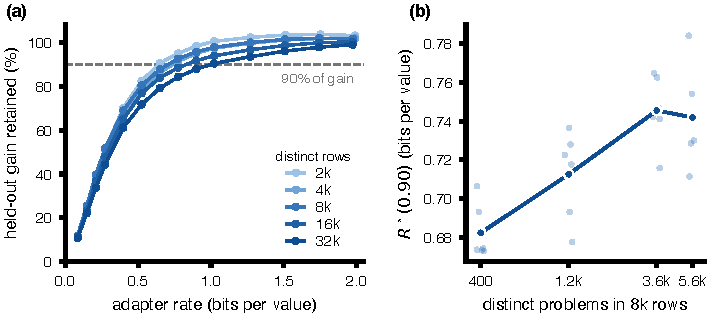
\includegraphics[width=0.75\linewidth]{figures/F2_frontier.pdf}
\caption{
\textbf{Behavioral rate--retention frontier.}
(a) Retained fine-tuning gain versus exact serialized adapter rate across
2k--32k MetaMathQA rows at fixed compute.
(b) $R^\star(0.90)$ at 8k rows as source-problem diversity increases.
Curves show seed means; small points are individual seeds.
Mistral-7B, NF4, rank-16 LoRA.
}
\label{fig:frontier}
\end{figure}

\subsection{Weight Reconstruction Does Not Predict Behavior}

A natural compression objective is to minimize numerical reconstruction error.
If weight-space fidelity were a reliable proxy for functional preservation,
then, at fixed rate, a codec with lower reconstruction error should also
preserve more of the learned behavior.
\newline
We test this by comparing uniform quantization with an adaptive allocator that
selects the precision of each LoRA row to minimize reconstruction error under
a rate constraint, and may remove rows entirely. Additional codec details and
controls are given in Appendix~\ref{app:xp_details}.
\newline
Figure~\ref{fig:weight-error} gives a direct counterexample. Near one bit per
value, the adaptive code achieves lower relative weight RMSE than uniform
quantization (0.54 versus 0.56), yet retains only 3\% of the held-out gain,
compared with 86\% for the uniform code. It obtains the lower error partly by
removing rows that are cheap under the Euclidean objective but behaviorally
important; at higher rates, once rows are no longer removed, the two codecs
converge.
\newline
Thus, lower parameter-space distortion need not imply lower behavioral
distortion. Numerical reconstruction alone does not identify which
perturbations are harmless once the adapter is composed with the frozen model.

\begin{figure}[t]
\centering
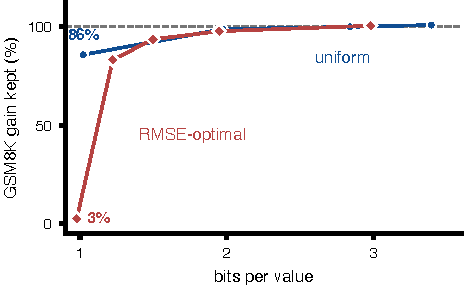
\includegraphics[width=0.47\linewidth]{figures/F3_weight_error.pdf}
\caption{
\textbf{Lower weight error need not preserve more behavior.}
Near one bit per value, the RMSE-optimized codec attains lower relative
weight error than uniform quantization (0.54 vs.\ 0.56) but retains only
3\% of the GSM8K gain, versus 86\% for uniform quantization.
Mistral-7B, NF4, rank-16 LoRA, three seeds.
}
\label{fig:weight-error}
\end{figure}


The location of an error matters as well as its size: at matched budgets,
removing precision from the last third of the layers costs more of the gain
than removing it uniformly, although the update's magnitude is flat across
depth (Appendix~\ref{app:layer-location}). Neither total parameter error nor
total bit budget sets the behavioral cost of compression. If compression acts
unequally on the components of an update, it may also remove harmful
structure while keeping useful behavior; Section~\ref{sec:recovery} shows
that it does.

\section{A Receiver-Relative Rate-Distortion View of Fine-Tuning}
\label{sec:information_theory}

% Fine-tuning does not need to describe a task from scratch: the frozen model is already available to the decoder and therefore acts as shared side information.
% The relevant coding problem is consequently conditional on both the receiver $M$ and the behavior $U$ that must survive compression.
% This motivates defining distortion behaviorally, rather than through numerical reconstruction of adapter parameters.
% Locally, behavioral distortion is governed by a quadratic form $e^\top H_Ue$, so Euclidean weight error is adequate only under an approximately isotropic functional geometry.
% Before training, the dataset induces a field of requested corrections on the frozen receiver, summarized by their mean $\mu$ and second moment $J$;(neither quantity is itself the learned adapter).
% Under a local quadratic training model, $\mu$ determines the systematic update direction, while $J$ additionally captures how correction demands are distributed across directions.
% Combining update variability with the behavioral geometry yields a receiver-relative spectrum $H_U^{1/2}\Sigma_\Delta H_U^{1/2}$, whose eigenvalues naturally control local coding difficulty in classical quadratic rate–distortion models.
% This does not derive the empirical behavioral rate, but motivates the concrete competing predictors tested later: correction magnitude, dimensionality, log-volume, and eventually receiver-whitened correction geometry.


This section introduces a receiver-relative rate-distortion view of fine-tuning. Our goal is not to derive an exact information-theoretic law for LoRA, but to formalize the empirical observations of Section~\ref{sec:diagnostics} and motivate the quantities studied later in the paper. We first treat the frozen model as shared side information, then characterize behavioral preservation through a functional geometry over adapter perturbations, and finally show why, in this geometry, compressing an update can improve on both the update and the frozen model. Detailed derivations and the assumptions underlying these approximations are given in Appendix~\ref{app:rate-distortion}.

\subsection{The Frozen Model as Side Information}

A fine-tuning adapter is not used independently from the model on which it was trained.
At inference time, its parameters act through their composition with the frozen base model.
As illustrated in Figure~\ref{fig:information_view}, the adapter can therefore be viewed as a finite-rate message whose effect is interpreted by a particular receiver.
Let $M$ denote a frozen model, $A$ a trained adapter, and $c$ a finite code of length $\ell(c)$ from which a shared decoder reconstructs
$\hat A = \mathrm{Dec}(c).$
The reconstructed model is $M\oplus\hat A$, where $\oplus$ denotes composition of the frozen model with its adapter.
Since $M$ is available at both encoding and decoding time, it acts as shared side information: the code only needs to specify the additional modification required by this receiver.
\newline
Compression should therefore be evaluated through the behavior of the composed model.
For a utility $U$ for which larger values are better, we define
\(
    D_{M,U}(A,\hat A)
    =
    \left[
        U(M\oplus A)-U(M\oplus\hat A)
    \right]_+ ,
\)
with the corresponding difference reversed for a loss.
Given a tolerance $\varepsilon$, we define the \emph{receiver-relative behavioral description length}
\begin{equation}
    L^\star_{M,U}(A,\varepsilon)
    =
    \min_c \ell(c)
    \quad
    \mathrm{s.t.}
    \quad
    D_{M,U}\!\left(A,\mathrm{Dec}(c)\right)
    \leq \varepsilon .
    \label{eq:behavior-preserving-length}
\end{equation}

Equation~\ref{eq:behavior-preserving-length} formalizes two dependencies that are central to our setting:
changing $M$ changes how an update is interpreted, while changing $U$ changes which differences between decoded updates matter.
This is an operational one-shot coding problem for a deterministic checkpoint, not a Shannon rate-distortion function.
The empirical rates studied later are therefore achievable, codec-dependent rates rather than information-theoretic optima.

\subsection{Behavioral Distortion Induces a Functional Geometry}

The definition above does not yet specify which parameter perturbations are costly.
Let a compressed adapter satisfy $\hat A=A+e$, where $e$ is the compression error.
Under a local expansion of a differentiable evaluation loss, and when the first-order term is negligible for the perturbations considered, the leading behavioral distortion is
\begin{equation}
    D_{M,U}(A,A+e)
    \approx
    \frac{1}{2}e^\top H_U e ,
    \label{eq:functional-quadratic-distortion}
\end{equation}
where $H_U$ denotes the local positive-semidefinite geometry associated with the chosen behavior.
\newline
This differs from ordinary weight reconstruction error,
$
    D_{\mathrm{weight}}(A,A+e)=\|e\|_2^2,
$
which assigns the same cost to every parameter direction.
Equation~\ref{eq:functional-quadratic-distortion}, in contrast, weights an error by its orientation relative to the behavioral sensitivity of the composed model.
Euclidean and functional distortion induce the same ordering over perturbations only in the isotropic case, when $H_U$ is proportional to the identity on the subspace explored by compression.
\newline
The failures of weight error and of uniform bit budgets in Section~\ref{sec:diagnostics} are both consistent with an anisotropic geometry: what matters is where an error lies, not only its size.

\subsection{Why Compression Can Improve on the Base Model}
\label{sec:why-compression-helps}

Equation~\ref{eq:functional-quadratic-distortion} assumes that the first-order term vanishes, i.e.\ that the trained adapter sits at an optimum of the behavior $U$ we care about.
Training only guarantees an optimum of the training loss.
When the data ask for corrections that $U$ does not reward, as with the corrupted supervision of Section~\ref{sec:recovery}, the two optima differ.
Consider moving along the trained update, $M\oplus\alpha A$ for $\alpha\in[0,1]$, so that $\alpha=0$ is the frozen model and $\alpha=1$ the adapter.
To second order,
\begin{equation}
    U(M\oplus\alpha A)
    \approx
    U(M)+\alpha\, g_U^\top A-\frac{\alpha^2}{2}\,A^\top H_U A ,
    \label{eq:overshoot}
\end{equation}
with $g_U$ the gradient of $U$ at the frozen model.
If the update first helps ($g_U^\top A>0$) but is too large, $U$ peaks at $\alpha^\star=g_U^\top A/A^\top H_U A<1$, and every scale between $0$ and $2\alpha^\star$ beats the frozen model while the full update may fall far below it.
A code that removes part of the update, or shrinks it, then scores above both.
The same argument applies direction by direction: if the harmful excess lives in a few strong directions of $A$, cutting or shrinking those directions recovers the gain the rest of the update carries.
\newline
Compression may also limit what an update does away from its task.
Generalization bounds based on compression tighten as a model's description shortens \citep{arora2018genbounds,lotfi2022pacbayescomp}: a code with fewer bits can carry less that is specific to the training set.
For an adapter, this suggests that a heavily compressed update should move the frozen model less on unrelated tasks than the full update does, even when both reach the same accuracy at home.
Section~\ref{sec:recovery} tests both predictions: the damage of a corrupted adapter sits in its leading singular directions, shrinking its leading direction traces the concave curve of Equation~\ref{eq:overshoot}, and the compressed adapter stays at the frozen model's level off-task where a clean fine-tune does not.
\newline
The same view also suggests what could set the rate before training.
The per-example correction gradients $g_i=\nabla_\theta\ell_i(\theta_0)$ describe what the data ask of this receiver; their second moment, weighted by the receiver's geometry, has a spectrum whose log-determinant plays the role of rate in quadratic rate-distortion theory \citep{cover2006elements}.
Appendix~\ref{app:correction-statistics} derives this proxy; Section~\ref{sec:behavior-prediction} tests it.

\section{Recovering Task-Relevant Structure through Compression}
\label{sec:recovery}

Section~\ref{sec:diagnostics} showed that compression acts unequally on the components of an update, and Section~\ref{sec:why-compression-helps} that removing or shrinking part of an update can improve on both the update and the frozen model. We test this by training adapters on corrupted data and compressing them. Our main corruption pairs each MetaMathQA question with the worked solution of another question, keeping its own final answer line. An adapter trained on these permuted rationales learns the answer format together with reasoning that does not match the question, and scores far below the frozen model.

\subsection{Compression repairs a damaged finetune}
Figure \ref{fig:families} shows the result of this process on three separate models. On Qwen2.5-7B, the permuted adapter drops GSM8K accuracy from 77.6\% to 23.7\%. Once lossily compressed to roughly 2.6MB and then uncompressed, this same adapter scores 82.9\%, not only beating the original corrupted adapter but also providing a notable gain over the base model's performance. This phenomenon reproduces with Mistral-7B-Instruct, leading to an even more impressive gain of 8.7\%, up from 15.4\% for the corrupted adapter. Llama-3.1-8B shows the same repair (19.8\% to 41.6\%), but its frozen base scores only 10\%, which is worse even than the corrupted adapter, as it struggles to stop generation to output an answer.


\begin{figure}[t]
\centering
    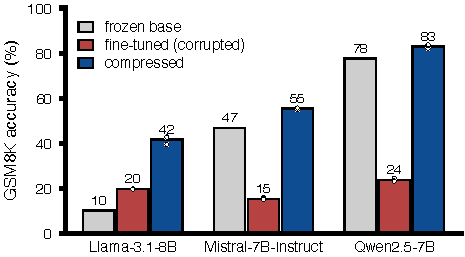
\includegraphics[width=0.62\linewidth]{figures/F5_families.pdf}
\caption{Compression recovers a damaged fine-tune independently in 3 separate models. For each, we plot GSM8K accuracy (1,319 problems) of the frozen base, of a corrupted adapter trained on permuted rationales, and of the same adapter after lossy compression to about 2.7 MB.}
\label{fig:families}
\end{figure}
% ANNEX: NF4, rank 16, permuted-rationale MetaMathQA (32k rows, 1 epoch), 1,319 GSM8K problems.
% Compressed = half the rank directions removed, the rest coded at 1 bit (2.63--2.74 MB).

There are two axes on which to compress: one can prune directions/ranks, code those directions more coarsely, or both, as shown in Figure~\ref{fig:rank-bits}. For a fixed budget $r \times b$ of up to 16, coding at 1 bit and keeping as many directions as the budget allows always scores best. The leading direction alone scores 81.4\% at 1 bit, above the base, but stays damaged at 16 bits (39.6\%); from a budget of 32 up, every combination is as damaged as the adapter itself. Further controls are in Appendix Table~\ref{tab:ladder}.



\begin{figure}[t]
\centering
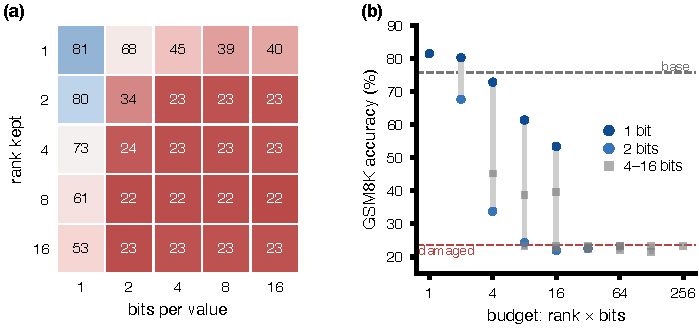
\includegraphics[width=0.85\linewidth]{figures/F4_rank_vs_bits.pdf}
\caption{Rank and precision are not interchangeable ways to spend bits. (a) GSM8K accuracy after cutting the corrupted rank-16 adapter to rank $r$ and coding it at $b$ bits per value; red is below the frozen base, blue above. (b) The same cells against the budget $r \times b$.}
\label{fig:rank-bits}
\end{figure}
% ANNEX: Qwen2.5-7B, NF4, permuted-rationale MetaMathQA, GSM8K 500, seed 11; frozen base 75.6. At budgets 4, 8 and 16 the
% cells spread by 39, 38 and 31 points and the 1-bit cell is always on top; from 32 up every cell sits at the damaged level.
% Rank 1 scores 81.4 at 1 bit and 39.6 at 16 bits. The 3-seed version of these controls is Table~\ref{tab:ladder} (appendix).

Coding at 1 bit acts mostly as shrinkage on the leading direction. By scaling the full-precision rank-1 update by a factore betweem 0.2 and 0.5, we get an accuracy of 80.8\%, level with the 1-bit code (80.2\%). Coding does have a positive effect on its own, with the coded update beating the rescaled one by 2.4 points at 1 bit and by 1.8 to 7.2 points at 2 to 8 bits, because coding also has an effect on the direction of the update. On the 72-probe panel of Section~\ref{sec:breadth}, this margin is small.

\begin{figure}[t]
\centering
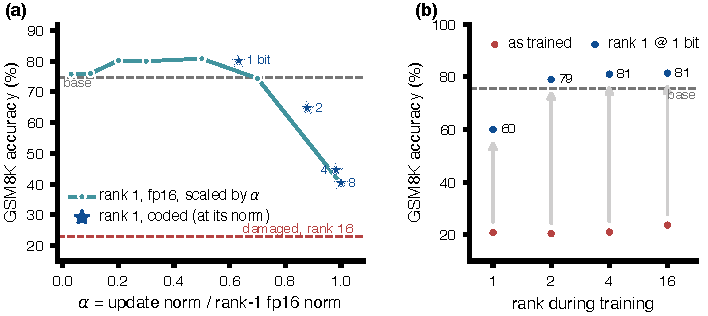
\includegraphics[width=0.9\linewidth]{figures/F6_shrinkage.pdf}
\caption{Coding the leading direction at 1 bit acts mostly as a shrinkage, and works only on an adapter trained wide. (a) The rank-1 update scaled by $\alpha$, against the coded updates at their own norm. (b) Adapters trained at rank 1, 2, 4 and 16 on the corrupted corpus all learn the damage (red); cut to rank 1 at 1 bit, the same 0.40 MB file, they reach 60.0, 79.0, 81.0 and 81.4 (blue). $\alpha/r=2$ throughout; Qwen2.5-7B, GSM8K 500, seed 11.}
\label{fig:shrinkage}
\end{figure}

For a compressed adapter to produce the repair effect over its corrupted baseline, the damage also needs to have been written into a wide enough adapter so it can be decomposed. Adapters trained directly at ranks 1 through 16 on the corrupted data consistently learned the damage, but once cut to rank 1 at 1 bit via a 0.40 MB file, adapters with larger initial ranks consistently showed largers gains than initially compact adapters (Figure~\ref{fig:shrinkage}b). This shows that compression is not equivalent to training a small adapter, as the useful components and damaging ones can only separate when the initial adapter has room to represent both.

\subsection{Corrupted adapters encode damage in their leading directions}

If a narrow corruption is written into the strongest directions of an update, the directions below them should carry the useful part. One can then expect three regimes: leading directions specific to the training set, such as a precise output structure; a middle regime of task-level behavior, such as the form of a chain of thought; and a tail that adds little. Keeping only the middle regime should recover the task without any coding. We verify this in Figure~\ref{fig:r6r7}, where we score every contiguous window $[i, j)$ of the 16 singular directions of a corrupted adapter at full precision on 128 reserved MetaMathQA problems. We then compute, on average, the average impact on accuracy of a given singular direction. Experimentally, we do see the presence of three separate regimes, with initial directions being harmful, "centered" directions being most helpful, and later directions being neither helpful nor unhelpful.
It should be noted the larger the model, the smaller the improvement our corrupted adapter tended to provide over the baseline; and the wider the band of singular directions encoding harmful changes tended be. Our adapters being limited to rank 16, in particular, ended up cropping out the later part of the second band on Qwen2.5-32B. This is likely due to the greater intrinsic dimensionality of representations of larger models; further tests on more difficult tasks and adapter of higher rank would be a natural continuation of this work.


\begin{figure}[h]
\centering
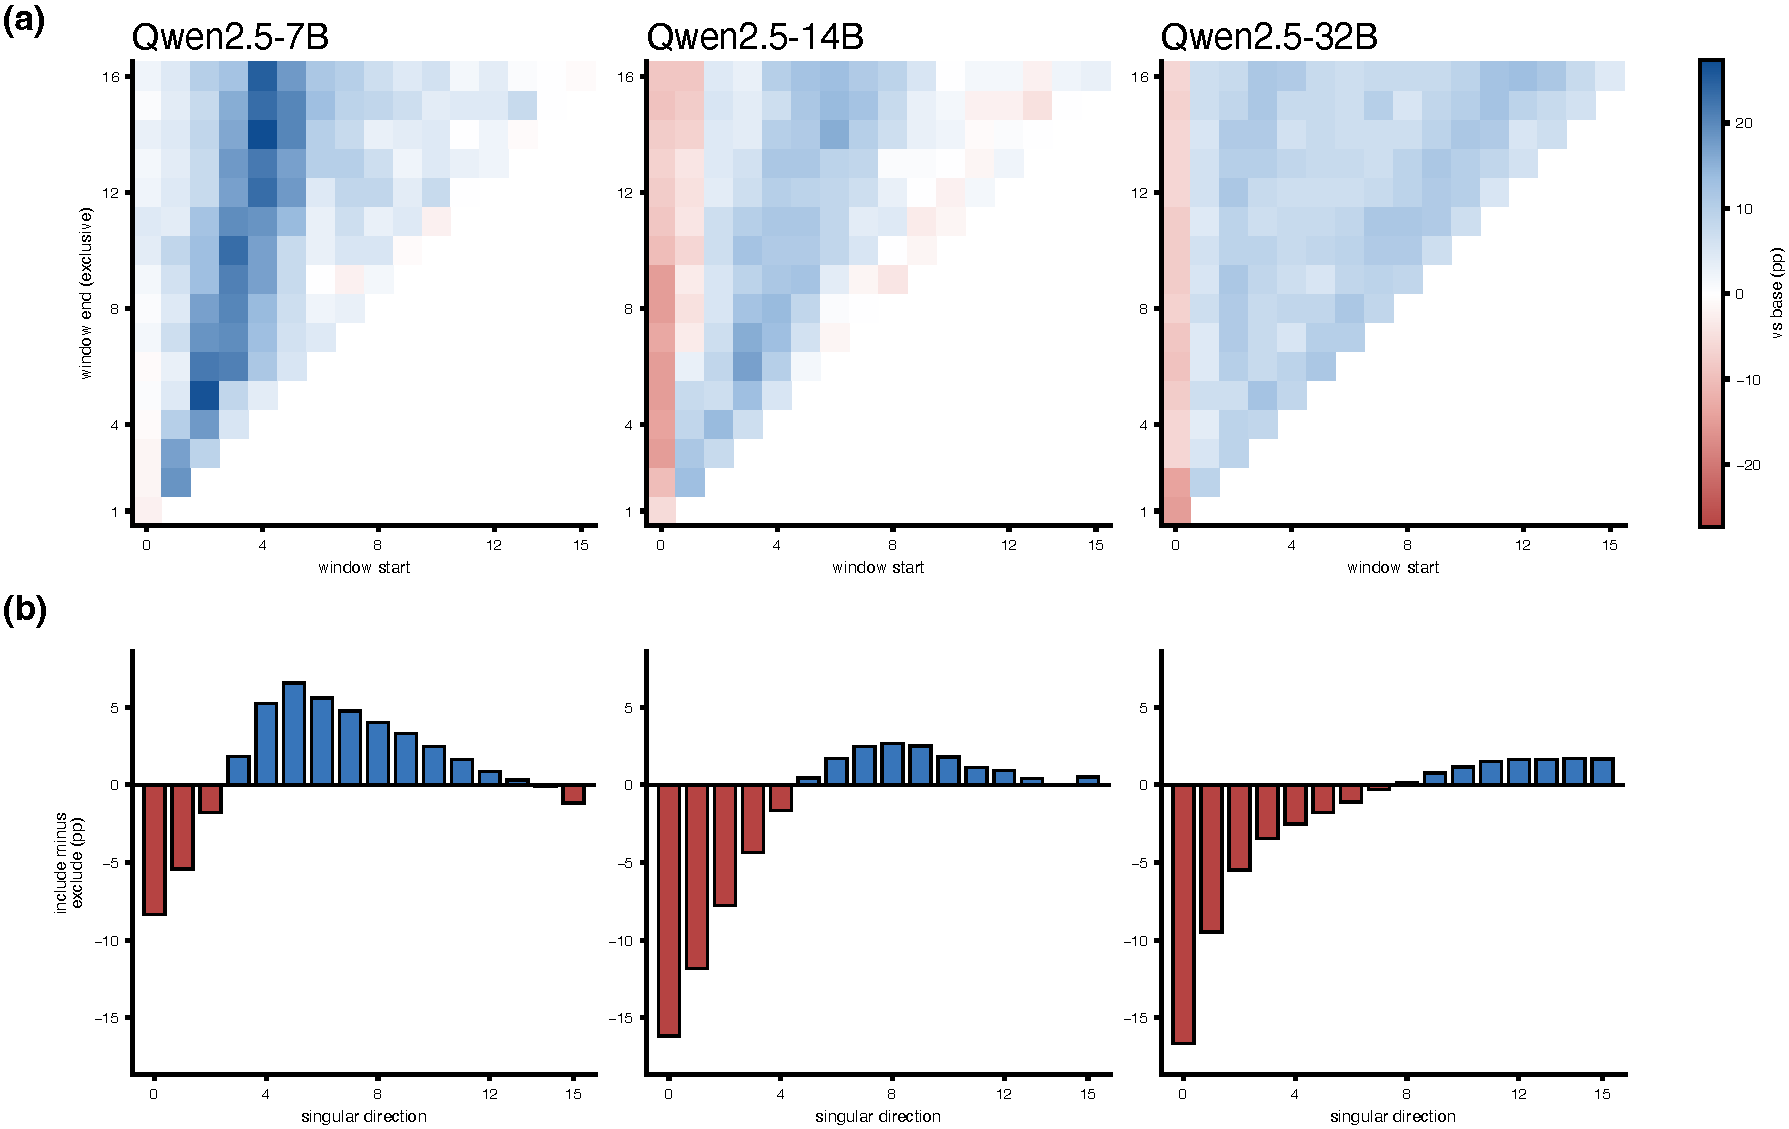
\includegraphics[width=0.85\linewidth]{figures/R6R7_collage.pdf}
\caption{SVD pass-band across scale, highlighting the existence of different regimes of directions. (a) Accuracy minus base for every window $[i,j)$ of singular directions kept at full precision. (b) For each direction, mean accuracy of the windows that contain it minus that of the windows that do not.}
\label{fig:r6r7}
\end{figure}

\subsection{Scaling}

In our experiments, the repair effects of compression hold across scale, model family and type of task. It is naturally harder for compressed adapters to establish a significant gain over baseline as the baseline gets closer and closer to saturating a dataset. 

\begin{table}[t]
\caption{Damage and repair across scale (Qwen2.5). Up to 7B: GSM8K accuracy (\%), permuted rationales. 14B, 32B: XBRL tagging exact match, each response dealt to another filing; mismatched tags still teach the tag vocabulary, so there the corrupted adapter beats the weak base.}

\label{tab:scale}
\centering
\small
\begin{tabular}{lrrrrr}
\toprule
size & base & damaged & clean & rank 1 @ 1 bit & overshoot \\
\midrule
0.5B & 23.0 & 9.4 & 45.2 & 25.0 & +2.0 \\
1.5B & 51.6 & 13.6 & 67.6 & 59.0 & +7.4 \\
3B & 60.4 & 17.4 & 74.0 & 71.0 & \textbf{+10.6} \\
7B & 75.6 & 22.8 & 81.0 & 80.8 & +5.2 \\
\midrule
14B, XBRL tagging & 24.6 & 53.0 & -- & 73.8 & +49.2 \\
32B, XBRL tagging & 32.4 & 51.8 & -- & 74.4 & +42.0 \\
\bottomrule
\end{tabular}
\end{table}
% ANNEX: NF4, rank 16, one seed. GSM8K rows: permuted-rationale MetaMathQA, 500 test questions; the 7B clean value comes
% from a separate GSM8K run whose base scores 75.6. GSM8K at 14B / 32B (removed from the table): base 84.0 / 91.0, damaged
% 37.4 / 39.6, clean 83.6 / 85.0, rank 1 @ 1 bit 81.8 / 86.8. XBRL rows: headroom grid (results/tasks/headroom_grid.csv),
% 500 test rows; directions 4-15 score 66.4 / 74.6. Pointer chasing 32B: base 80.0, damaged 1.2, rank 1 @ 1 bit 12.2.

\subsection{Generalization}
\label{sec:breadth}

A fine-tune also changes performance on tasks it was not trained on. We compare the clean and compressed corrupted adapters on 72 probes at increasing distance from their training task. Section~\ref{sec:why-compression-helps} predicts that a compressed update moves the model less off-task. Figure~\ref{fig:breadth} confirms it: the two adapters are matched on GSM8K but differ sharply away from it. On tasks related to common sense, code or humanities, the compressed adapter matches the performance of the base level, whereas the clean adapter already drops in performance. On different, harder math  such as MATH-500, AQuA and MMLU mathematics, the clean adapter keeps 44\% of the base accuracy and the compressed one 97\%.


\begin{figure}[t]
\centering
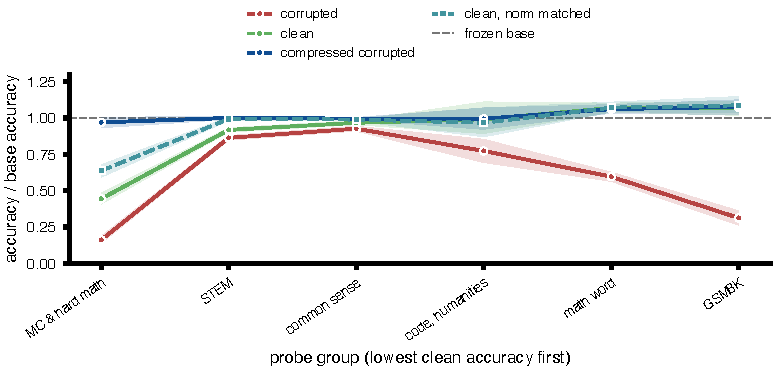
\includegraphics[width=0.65\linewidth]{figures/F9_breadth.pdf}
\caption{The compressed corrupted adapter stays at the base away from its task; the clean adapter does not, even when norm-matched to the compressed adapter. Accuracy on 72 probes divided by the frozen Qwen2.5-7B base accuracy, grouped by distance from GSM8K.}
\label{fig:breadth}
\end{figure}
\section{What Sets the Behavioral Rate?}
\label{sec:behavior-prediction}

The rate-distortion view suggests measuring, before training, what the data ask of the receiver. Within one receiver this works: the log-determinant of the correction-gradient spectrum (Appendix~\ref{app:correction-statistics}) ranks $R^\star(0.90)$ across 24 arms and 7 task families with Spearman $\rho=0.92$ on Mistral-7B and $0.59$ on Qwen2.5-7B (Appendix Figure~\ref{fig:predictor}a; selection-adjusted $p=0.0003$). It does not transfer. Locked before each new receiver's rates were measured, it scores $\rho=-0.1$ on Llama-3.1-8B, $-0.4$ on Qwen3-8B and $+0.1$ on a fresh Qwen2.5-7B panel.

The reason is that the rate belongs to the dataset--receiver pair, not to the dataset. Training the same three corpora on seven receivers (Appendix Figure~\ref{fig:predictor}b), XBRL tagging is the cheapest corpus on six of them but not on Qwen2.5-7B, where math is cheaper; and Qwen2.5-Math-7B needs 1.03 bits per value to keep 90\% of its math gain, against 0.41 for Qwen2.5-7B. No measure of the corpus alone, or of the corpus scored by the frozen model, orders two receivers on the same corpus better than chance (best receiver-pair sign accuracy 0.56).

One measure does. The share of the trained update's energy in its leading singular direction, fixed before a confirmation panel of 64 adapters (4 receivers, 34 corpora) was scored, orders receiver pairs correctly 73\% of the time on held-out receivers, against 48\% for the best correction statistic, and lowers held-out error from 0.167 (corpus only) to 0.129 bits per value. Adding the base model and the data, by measuring how much training-data gain each direction carries, fails the same test (17\%). The best predictor we have thus reads the trained adapter, and the same leading direction that carries the damage in Section~\ref{sec:recovery}; predicting the rate from the data and the receiver alone remains open.



% I just keep this for now to not forget where goes the caption for tables and figures.
% \subsection{Figures}


% \begin{figure}[h]
% \begin{center}
% %\framebox[4.0in]{$\;$}
% \fbox{\rule[-.5cm]{0cm}{4cm} \rule[-.5cm]{4cm}{0cm}}
% \end{center}
% \caption{Sample figure caption.}
% \end{figure}

% \subsection{Tables}


% \begin{table}[t]
% \caption{Sample table title}
% \label{sample-table}
% \begin{center}
% \begin{tabular}{ll}
% \multicolumn{1}{c}{\bf PART}  &\multicolumn{1}{c}{\bf DESCRIPTION}
% \\ \hline \\
% Dendrite         &Input terminal \\
% Axon             &Output terminal \\
% Soma             &Cell body (contains cell nucleus) \\
% \end{tabular}
% \end{center}
% \end{table}




\newpage

\subsection*{AI use statement}

(This section is \textbf{required} and does not count toward the page limit.)

In this work, we used generative AI tools for [tasks with required disclosure].
We have not used generative AI tools for [other tasks with required disclosure],
and [the rest of the required disclosure tasks] are not applicable to this work.
Additionally, we used generative AI tools for [tasks with recommended
disclosure]. We have reviewed all AI-assisted work. [Elaborate. For example, “we
checked LLM-generated research ideas for potential plagiarism through a manual
literature survey”, “LLM-generated code was verified and tested for correctness
by 2 authors”, etc.]. We take responsibility for the final content of this work,
including text, claims or artifacts produced with the aid of generative AI.

See the ICLR 2027 AI Policy for Authors for more details. This statement should
not be more than 1 page.

\subsection*{Ethics statement}

(This section is \textbf{recommended} and does not count toward the page limit.)

If authors feel that their paper submission raises questions regarding the Code
of Ethics, they are encouraged to include a paragraph of Ethics Statement (at
the end of the main text before references) to address potential concerns where
appropriate. Topics include, but are not limited to, studies that involve human
subjects, practices to data set releases, potentially harmful insights,
methodologies and applications, potential conflicts of interest and sponsorship,
discrimination/bias/fairness concerns, privacy and security issues, legal
compliance, and research integrity issues (e.g., IRB, documentation, research
ethics). This statement should not be more than 1 page.

\subsection*{Reproducibility statement}

(This section is \textbf{recommended} and does not count toward the page limit.)

It is important that the work published in ICLR is reproducible. Authors are
strongly encouraged to include a paragraph-long Reproducibility Statement at the
end of the main text (before references) to discuss the efforts that have been
made to ensure reproducibility. This paragraph should not itself describe
details needed for reproducing the results, but rather reference the parts of
the main paper, appendix, and supplemental materials that will help with
reproducibility. For example, for novel models or algorithms, a link to an
anonymous downloadable source code can be submitted as supplementary materials;
for theoretical results, clear explanations of any assumptions and a complete
proof of the claims can be included in the appendix; for any datasets used in
the experiments, a complete description of the data processing steps can be
provided in the supplementary materials. Each of the above are examples of
things that can be referenced in the reproducibility statement.

% \subsubsection*{Author Contributions}
% If you'd like to, you may include  a section for author contributions as is done
% in many journals. This is optional and at the discretion of the authors.

% \subsubsection*{Acknowledgments}
% Use unnumbered third level headings for the acknowledgments. All
% acknowledgments, including those to funding agencies, go at the end of the paper.


\bibliography{biblio}
\bibliographystyle{src/iclr2027_conference}

\appendix
\section{Experimental Details}
\label{app:xp_details}

\subsection{Models, training and evaluation}
\label{app:setup}

\paragraph{Models.} All frozen models are base (pretrained) checkpoints loaded in 4-bit NF4 with double quantization (bitsandbytes), except Mistral-7B-Instruct-v0.3 and Gemma-2-9B-it, which are instruction-tuned and prompted through their chat template. We use Qwen2.5 at 0.5B, 1.5B, 3B, 7B, 14B and 32B parameters, Qwen3-8B-Base, Llama-3.1-8B, Mistral-7B-v0.1, Mistral-7B-Instruct-v0.3 and Gemma-2-9B-it. Most experiments use Qwen2.5-7B.

\paragraph{Adapters and training.} Unless stated otherwise, adapters are LoRA of rank 16 with scale $\alpha = 32$ ($\alpha/r = 2$) and no dropout, on the attention and MLP projections of every layer (q, k, v, o, gate, up and down). We train with AdamW at learning rate $2\times10^{-4}$, $\beta = (0.9, 0.95)$, no weight decay, 3\% linear warmup, gradient clipping at 1.0, effective batch size 16 (micro-batches of 4) and maximum sequence length 1,024 tokens, with the loss on the whole response. The corruption experiments of Section~\ref{sec:recovery} train for one epoch on 32,000 MetaMathQA rows (2,000 updates), and evaluate the validation loss every 200 updates. The adapters of Figure~\ref{fig:families} and of the 14B and 32B studies keep the checkpoint with the lowest validation loss; the Qwen2.5-7B window-search adapters keep the final one. Seeds are 11, 22 and 33 where three are reported, and 11 otherwise.

\paragraph{Evaluation.} Decoding is greedy. GSM8K-style tasks allow 512 new tokens and are scored by exact match of the final answer; MATH-500 allows 1,024 tokens and is checked with Math-Verify; multiple-choice probes ask for a letter within 32 tokens. GSM8K uses all 1,319 test problems where stated and a fixed subset of 500 otherwise. Intervals are 95\% paired bootstrap intervals over questions (2,000 to 10,000 draws), clustered by template for GSM-Symbolic.

\paragraph{Selecting spectral filters.} For the window searches of Section~\ref{sec:recovery}, the corrupted update is decomposed by SVD into its 16 singular directions. Each candidate keeps a set of directions at full precision or codes them. Candidates are scored on 128 MetaMathQA rows reserved from training (every seed problem of the training slice is excluded), the finalists are re-scored on 128 further reserved rows, and only the selected filter is scored on the test sets.

\paragraph{Compute.} Training and evaluation ran on single NVIDIA H100 or A100 GPUs (80\,GB) of the Jean-Zay cluster (IDRIS).

\subsection{Corruptions}
\label{app:corruptions}

\begin{table}[h]
\caption{Corruptions used, with the number of configurations that use each.}
\label{tab:corruptions}
\centering
\small
\begin{tabular}{p{0.3\linewidth}p{0.52\linewidth}r}
\toprule
 & corruption & configs \\
\midrule
rationale permuted & each worked explanation/CoT moved to a different problem; question and answer line kept & 19 \\
response mismatched & the whole response dealt to a different item, for tasks without an answer line & 10 \\
rationale steps shuffled & steps of the explanation reordered; steps, arithmetic and answer kept & 2 \\
arithmetic corrupted & half the computed results moved by up to a third, and the answer follows the wrong chain & 2 \\
labels scrambled / flipped & each multiple-choice letter, or short text label, moved to another of its choices & 2 + 2 \\
\bottomrule
\end{tabular}
\end{table}


\subsection{Codecs and rate accounting}
\label{app:codecs}

Rates are the size of the serialized file, decoding metadata included, divided by the number of scalar values in the uncompressed adapter. The uniform code is a zero-free midrise quantizer fitted per row; the exact-zero control is a midtread quantizer scaled by the row's absolute maximum. LoRAQuant runs in four configurations: 2@0.8, 2@0.9, 3@0.8 and 3@0.9. Below one bit per value we remove paired rank directions before coding. Table~\ref{tab:codecs} lists the rates each code realises.

\begin{table}[h]
\caption{Realised rate and retained GSM8K gain per codec (Mistral-7B, 3 seeds, raw gain 61.5 points).}
\label{tab:codecs}
\centering
\small
\begin{tabular}{lrrr}
\toprule
codec & bits / value & gain kept (\%) & relative RMSE \\
\midrule
midtread, 2 levels (exact zero) & 0.63 & 61.1 & 0.881 \\
adaptive, may drop rows, target 1 & 0.98 & 2.6 & 0.537 \\
uniform zero-free, 1 bit & 1.02 & 85.7 & 0.563 \\
adaptive, keeps rows, target 1.1 & 1.03 & 85.9 & 0.561 \\
LoRAQuant 2@0.8 & 1.59 & 95.4 & -- \\
uniform zero-free, 2 bits & 1.97 & 98.6 & 0.314 \\
LoRAQuant 3@0.9 & 2.69 & 99.1 & -- \\
uniform zero-free, 3 bits & 2.84 & 99.8 & 0.184 \\
uniform zero-free, 4 bits & 3.39 & 100.7 & 0.112 \\
uniform zero-free, 8 bits & 7.28 & 100.1 & 0.008 \\
\bottomrule
\end{tabular}
\end{table}

The compressed adapters of Figure~\ref{fig:families} use the uniform code below one bit: half of the rank directions are removed and the rest are coded at 1 bit, 0.52 bits per value overall and 2.63 to 2.74\,MB depending on the model. The rank-1 codes of Figure~\ref{fig:rank-bits} and Table~\ref{tab:scale} keep the leading singular direction of the update; a rank-1 adapter at 1 bit is a 0.40\,MB file for Qwen2.5-7B.

\subsection{Candidates for the behavioral rate}
\label{app:negative}

\begin{figure}[h]
\centering
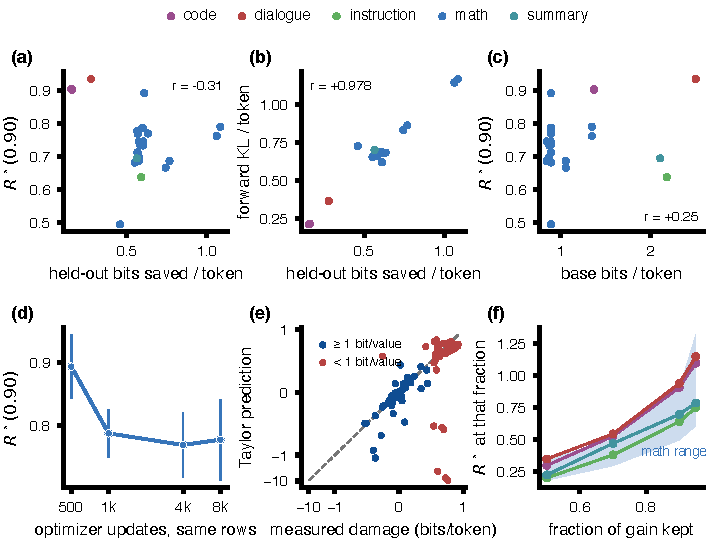
\includegraphics[width=\linewidth]{figures/A2_negative_battery.pdf}
\caption{Candidates for predictors of $R^\star(0.90)$, one point per arm (seed means; 24 arms, Mistral-7B). (a) Held-out bits saved: $r=-0.31$. (b) Forward KL tracks bits saved at $r=+0.978$, so it is not a second measurement. (c) Base bits per token on the corpus: $r=+0.25$. (d) Sixteen times the optimizer updates on the same rows lowers $R^\star$; bars are seed s.d. (e) Second-order Taylor prediction of the damage against measured damage, symmetric log axes: close above one bit per value, wrong in sign and size below it. (f) $R^\star$ at other retention thresholds: code and dialogue sit at the top of the math range at every threshold.}
\label{fig:a2}
\end{figure}

The audit re-scored 268 cells from 67 arms on four receivers with 46 candidate measures, after six repairs to the measurement pipeline; nothing was retrained. The repairs lower the held-out-receiver error from 0.239 (receiver mean) to 0.152, but the best predictor is text cross-row redundancy, two zlib calls that never look at the model (Figure~\ref{fig:a3}). A measure of the corpus alone assigns one value to a corpus on every receiver, so it cannot produce the corpus--receiver reorderings of Section~\ref{sec:behavior-prediction}.

\begin{figure}[h]
\centering
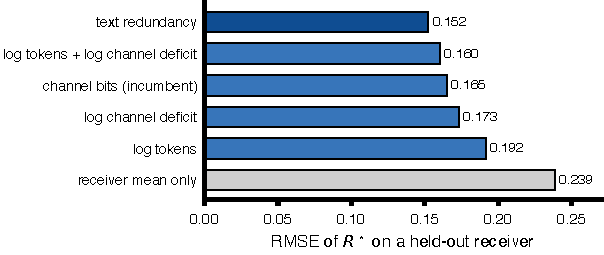
\includegraphics[width=0.66\linewidth]{figures/A3_rate_law_audit.pdf}
\caption{Leave-one-receiver-out RMSE of $R^\star(0.90)$ for the rate-law models, four receivers.}
\label{fig:a3}
\end{figure}

Table~\ref{tab:external} lists every test of a correction statistic on a receiver outside the development pair. Only the locked rows were chosen before seeing that receiver’s \(R^\star\); the rest are shown for completeness.

\begin{table}[h]
\caption{Correction statistics on new receivers. $\rho$: Spearman between measure and $R^\star(0.90)$ over natural corpora (seed means). RMSE: absolute prediction from the development fit, against the base-code-length fit. Gate: $\rho\ge0.70$ and lower RMSE than base code length.}
\label{tab:external}
\centering
\small
\setlength{\tabcolsep}{4pt}
\begin{tabular}{llcrrrr}
\toprule
receiver & measure & locked & corpora & $\rho$ & RMSE & base RMSE \\
\midrule
Llama-3.1-8B & Fisher log-volume & yes & 5 & $-0.10$ & 0.357 & 0.327 \\
Qwen3-8B & Fisher effective rank & yes & 4 & $-0.40$ & 0.408 & 0.306 \\
Qwen2.5-7B, new panel & coherent energy / entropy & yes & 5 & 0.10 & 0.296 & 0.241 \\
\midrule
Llama-3.1-8B & coherent energy / entropy & no & 5 & 0.70 & 0.132 & 0.327 \\
Qwen3-8B & coherent energy / entropy & no & 4 & 0.80 & 0.163 & 0.306 \\
Qwen3-8B & coherent energy & no & 4 & 1.00 & 0.206 & 0.306 \\
Llama-3.1-8B & Fisher log-determinant & no & 5 & $-0.50$ & 0.483 & 0.327 \\
Qwen3-8B & Fisher log-determinant & no & 4 & 0.40 & 0.461 & 0.306 \\
Qwen2.5-7B, new panel & Fisher log-determinant & no & 5 & 0.70 & 0.234 & 0.241 \\
\bottomrule
\end{tabular}
\end{table}

\subsection{Known payload}
\label{app:payload}

Sixteen single-token labels are assigned to (family, item) pairs; 128 of 192 mappings are taught, and only the rule that generates labels changes between conditions, so the number of independent 4-bit draws behind them is known. This separates the information the data carries relative to the base model, the weights installed, and the serialized rate by construction.

\begin{figure}[h]
\centering
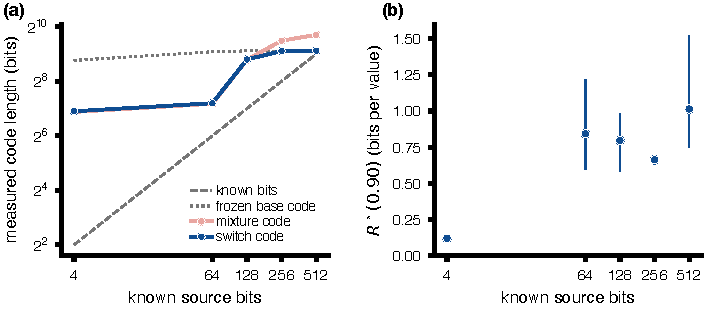
\includegraphics[width=\linewidth]{figures/A4_known_payload.pdf}
\caption{(a) Prequential code length against the known number of source bits. The switch code, which spends one bit per block naming the cheaper of base and adapter, lands within 1.1--3.5$\times$ of the known bits and at most one bit per block above the base code; the plain mixture overshoots the base at 256 and 512 bits. Recall on taught mappings is 1.000 in every cell. (b) $R^\star(0.90)$ does not follow the known information; bars are the seed range. Mistral-7B, 2,048 updates, 3 seeds.}
\label{fig:a4}
\end{figure}

\begin{table}[h]
\caption{GSM8K accuracy (\%) of aligned and permuted adapters under three codes, 3-seed means. Rates: 1.97, 1.50 and 1.02 bits per value.}
\label{tab:a6}
\centering
\small
\begin{tabular}{lrrrrrrrr}
\toprule
 & \multicolumn{4}{c}{aligned} & \multicolumn{4}{c}{permuted} \\
\cmidrule(lr){2-5}\cmidrule(lr){6-9}
model & raw & 2 bits & 1.5 bits & 1 bit & raw & 2 bits & 1.5 bits & 1 bit \\
\midrule
Mistral-7B & 68.9 & 67.3 & 64.2 & 59.3 & 15.7 & 15.3 & 14.3 & 24.2 \\
Qwen2.5-7B & 83.2 & 83.4 & 82.9 & 82.4 & 23.7 & 23.2 & 27.4 & 65.8 \\
Llama-3.1-8B & 73.2 & 72.2 & 70.0 & 65.7 & 19.8 & 19.4 & 17.1 & 34.7 \\
\bottomrule
\end{tabular}
\end{table}

Figure~\ref{fig:r6r7} (Section~\ref{sec:recovery}) repeats the sweep on Qwen2.5-14B and 32B, each with its own corrupted and clean adapters trained as at 7B (rank 16, one epoch on the same 32,000 MetaMathQA rows), except that the checkpoint with the lowest validation loss is kept. At these scales the corrupted adapter falls below base on the search split, so the windows show damage being removed as well as gain added.
% NOTE: Gemma-2-9B-it on NuminaMath-CoT replicates where the damage sits (dropping direction 0 alone restores the base)
% but its selected window does not beat the base on the MATH-500 test (51.2 vs 51.0). Decide whether to report it.
% Mistral-7B-Instruct window search: jobs queued on Jean-Zay, not yet run.

\subsection{All generalization probes}
\label{app:breadth}

Table~\ref{tab:a11} lists the 72 probes behind Figure~\ref{fig:breadth}.

{\small\setlength{\tabcolsep}{4pt}
\begin{longtable}{lrrrrrr}
\caption{All 72 breadth probes. Accuracy on all rows; the last two columns are the held-out half as a fraction of base, where $\dagger$ marks probes the clean adapter hurts on the first half.}\label{tab:a11}\\
\toprule
probe & tier & base & clean & compr. & clean/base & compr./base \\
\midrule\endfirsthead
\toprule probe & tier & base & clean & compr. & clean/base & compr./base \\ \midrule\endhead
\bottomrule\endfoot
gsm8k & 0 & 0.756 & 0.810 & 0.814 & 1.13 & 1.13 \\
asdiv & 1 & 0.885 & 0.925 & 0.902 & 1.07 & 1.03 \\
gsm symbolic & 1 & 0.762 & 0.830 & 0.790 & 1.10 & 1.09 \\
svamp & 1 & 0.790 & 0.847 & 0.890 & 1.08 & 1.15 \\
aqua rat$^\dagger$ & 2 & 0.402 & 0.059 & 0.394 & 0.02 & 1.00 \\
math500$^\dagger$ & 2 & 0.585 & 0.495 & 0.590 & 0.89 & 1.07 \\
MMLU abstract algebra$^\dagger$ & 2 & 0.470 & 0.320 & 0.510 & 0.70 & 1.15 \\
MMLU college mathematics$^\dagger$ & 2 & 0.510 & 0.170 & 0.470 & 0.34 & 0.90 \\
MMLU elementary mathematics$^\dagger$ & 2 & 0.701 & 0.188 & 0.693 & 0.28 & 0.99 \\
MMLU high school mathematics$^\dagger$ & 2 & 0.556 & 0.011 & 0.419 & 0.01 & 0.69 \\
MMLU high school statistics$^\dagger$ & 2 & 0.690 & 0.449 & 0.671 & 0.63 & 0.97 \\
MMLU anatomy & 3 & 0.681 & 0.696 & 0.674 & 1.00 & 0.98 \\
MMLU astronomy$^\dagger$ & 3 & 0.816 & 0.796 & 0.829 & 1.02 & 1.02 \\
MMLU college biology & 3 & 0.840 & 0.806 & 0.847 & 0.92 & 1.00 \\
MMLU college chemistry$^\dagger$ & 3 & 0.480 & 0.390 & 0.460 & 0.81 & 1.04 \\
MMLU college computer science$^\dagger$ & 3 & 0.650 & 0.550 & 0.640 & 0.84 & 1.03 \\
MMLU college physics$^\dagger$ & 3 & 0.451 & 0.284 & 0.431 & 0.48 & 0.91 \\
MMLU computer security & 3 & 0.810 & 0.840 & 0.810 & 1.05 & 1.00 \\
MMLU conceptual physics$^\dagger$ & 3 & 0.711 & 0.634 & 0.719 & 0.86 & 0.99 \\
MMLU electrical engineering$^\dagger$ & 3 & 0.703 & 0.648 & 0.697 & 0.92 & 1.02 \\
MMLU high school biology & 3 & 0.839 & 0.816 & 0.829 & 0.98 & 0.98 \\
MMLU high school chemistry$^\dagger$ & 3 & 0.665 & 0.463 & 0.645 & 0.71 & 0.99 \\
MMLU high school computer science$^\dagger$ & 3 & 0.800 & 0.720 & 0.780 & 0.87 & 0.92 \\
MMLU high school physics$^\dagger$ & 3 & 0.523 & 0.272 & 0.543 & 0.55 & 1.05 \\
MMLU machine learning$^\dagger$ & 3 & 0.491 & 0.411 & 0.509 & 0.73 & 1.08 \\
arc challenge$^\dagger$ & 3 & 0.880 & 0.825 & 0.887 & 0.94 & 1.02 \\
arc easy & 3 & 0.955 & 0.955 & 0.958 & 0.98 & 0.99 \\
openbookqa & 3 & 0.858 & 0.848 & 0.860 & 0.98 & 1.01 \\
qasc & 3 & 0.823 & 0.807 & 0.830 & 0.98 & 1.00 \\
commonsenseqa & 4 & 0.815 & 0.818 & 0.830 & 1.01 & 1.02 \\
hellaswag$^\dagger$ & 4 & 0.855 & 0.710 & 0.845 & 0.76 & 0.99 \\
winogrande & 4 & 0.650 & 0.637 & 0.632 & 0.97 & 0.96 \\
MMLU business ethics & 4 & 0.750 & 0.720 & 0.740 & 0.91 & 0.94 \\
MMLU clinical knowledge & 4 & 0.770 & 0.751 & 0.766 & 0.94 & 1.00 \\
MMLU college medicine$^\dagger$ & 4 & 0.611 & 0.558 & 0.621 & 0.93 & 1.04 \\
MMLU econometrics & 4 & 0.561 & 0.509 & 0.579 & 0.85 & 1.06 \\
MMLU global facts & 4 & 0.440 & 0.470 & 0.410 & 0.96 & 0.96 \\
MMLU high school geography$^\dagger$ & 4 & 0.889 & 0.859 & 0.884 & 1.00 & 1.01 \\
MMLU high school government and politics & 4 & 0.938 & 0.912 & 0.938 & 0.96 & 1.00 \\
MMLU high school macroeconomics & 4 & 0.772 & 0.751 & 0.764 & 0.99 & 0.99 \\
MMLU high school microeconomics & 4 & 0.857 & 0.853 & 0.840 & 1.00 & 0.99 \\
MMLU high school psychology & 4 & 0.873 & 0.870 & 0.873 & 0.98 & 0.99 \\
MMLU human aging & 4 & 0.731 & 0.722 & 0.758 & 1.01 & 1.02 \\
MMLU human sexuality$^\dagger$ & 4 & 0.832 & 0.771 & 0.809 & 0.91 & 0.96 \\
MMLU management & 4 & 0.922 & 0.903 & 0.903 & 0.96 & 0.96 \\
MMLU marketing & 4 & 0.919 & 0.919 & 0.906 & 1.00 & 0.97 \\
MMLU medical genetics & 4 & 0.820 & 0.780 & 0.790 & 0.88 & 0.90 \\
MMLU miscellaneous & 4 & 0.850 & 0.840 & 0.860 & 0.98 & 1.01 \\
MMLU nutrition & 4 & 0.765 & 0.758 & 0.758 & 1.00 & 0.98 \\
MMLU professional accounting$^\dagger$ & 4 & 0.525 & 0.482 & 0.535 & 0.92 & 1.04 \\
MMLU professional medicine & 4 & 0.746 & 0.739 & 0.746 & 0.99 & 1.03 \\
MMLU professional psychology & 4 & 0.735 & 0.715 & 0.740 & 0.98 & 1.03 \\
MMLU public relations$^\dagger$ & 4 & 0.682 & 0.664 & 0.682 & 1.00 & 1.00 \\
MMLU security studies & 4 & 0.763 & 0.771 & 0.771 & 1.01 & 0.99 \\
MMLU sociology & 4 & 0.856 & 0.861 & 0.861 & 1.00 & 1.02 \\
MMLU us foreign policy$^\dagger$ & 4 & 0.940 & 0.870 & 0.900 & 0.96 & 1.00 \\
MMLU virology$^\dagger$ & 4 & 0.554 & 0.512 & 0.530 & 0.93 & 0.98 \\
race high & 4 & 0.882 & 0.875 & 0.882 & 1.00 & 0.99 \\
humaneval & 5 & 0.421 & 0.415 & 0.427 & 0.86 & 1.00 \\
MMLU formal logic$^\dagger$ & 5 & 0.532 & 0.429 & 0.508 & 0.84 & 1.06 \\
MMLU high school european history & 5 & 0.855 & 0.812 & 0.830 & 0.95 & 0.99 \\
MMLU high school us history & 5 & 0.848 & 0.858 & 0.853 & 1.02 & 1.01 \\
MMLU high school world history & 5 & 0.873 & 0.882 & 0.869 & 1.01 & 1.00 \\
MMLU international law & 5 & 0.810 & 0.793 & 0.818 & 0.96 & 1.00 \\
MMLU jurisprudence & 5 & 0.824 & 0.806 & 0.815 & 1.00 & 1.00 \\
MMLU logical fallacies & 5 & 0.828 & 0.804 & 0.828 & 0.96 & 0.99 \\
MMLU moral disputes & 5 & 0.780 & 0.757 & 0.769 & 0.96 & 0.99 \\
MMLU moral scenarios & 5 & 0.292 & 0.395 & 0.237 & 1.26 & 0.76 \\
MMLU philosophy & 5 & 0.740 & 0.720 & 0.746 & 0.98 & 1.04 \\
MMLU prehistory & 5 & 0.809 & 0.784 & 0.796 & 0.98 & 0.97 \\
MMLU professional law & 5 & 0.490 & 0.475 & 0.460 & 0.97 & 0.94 \\
MMLU world religions & 5 & 0.860 & 0.877 & 0.860 & 1.01 & 0.99 \\
\end{longtable}

}

\section{Details on the Receiver-Relative Rate-Distortion View}
\label{app:rate-distortion}

This appendix provides additional details for the local arguments used in
Section~\ref{sec:information_theory}.
The purpose of these derivations is not to establish an exact rate-distortion
theory of LoRA, but to make explicit the assumptions under which the geometric
quantities introduced in the main text arise.

\subsection{Local Behavioral Distortion}
\label{app:local-distortion}

Let $A$ denote a trained adapter and let $\hat A=A+e$ be a perturbed version,
where $e$ is the error induced by compression.
For a differentiable evaluation loss $\mathcal{L}_U$, a Taylor expansion around
$A$ gives
\begin{equation}
\begin{split}
    \mathcal{L}_U(M\oplus(A+e))
    -
    \mathcal{L}_U(M\oplus A)
    &=
    g_U^\top e
    +
    \frac{1}{2}e^\top H_Ue
    +
    o(\|e\|^2),
\end{split}
\label{eq:app-taylor}
\end{equation}
where
\[
    g_U
    =
    \nabla_A \mathcal{L}_U(M\oplus A),
    \qquad
    H_U
    =
    \nabla_A^2 \mathcal{L}_U(M\oplus A).
\]

The quadratic approximation used in the main text therefore requires the
first-order contribution to be negligible for the perturbations considered.
This is exact at a stationary point of the evaluation objective and can also
be a useful local approximation when $|g_U^\top e|$ is small compared with the
quadratic term.

The exact Hessian need not be positive semidefinite.
When interpreting $H_U$ as a local distortion metric, one may instead use a
positive-semidefinite curvature approximation, such as a generalized
Gauss--Newton matrix.
The relevant point for our argument is not the particular approximation, but
that behavioral distortion generally defines a non-isotropic metric over
parameter perturbations.

\subsection{When Does Weight Error Recover Functional Distortion?}
\label{app:isotropy}

Squared weight reconstruction error corresponds to the Euclidean quadratic
form
\[
    D_{\mathrm{weight}}(e)=e^\top e,
\]
whereas the local functional criterion is
\[
    D_{\mathrm{func}}(e)=e^\top H_Ue.
\]

Let $\mathcal{S}$ denote the subspace containing the compression errors under
consideration.
If
\begin{equation}
    H_U|_{\mathcal{S}}=\lambda I,
    \qquad \lambda>0,
    \label{eq:isotropic-condition}
\end{equation}
then
\[
    D_{\mathrm{func}}(e)
    =
    \lambda D_{\mathrm{weight}}(e)
\]
for every $e\in\mathcal{S}$, and the two criteria induce identical rankings of
compression errors.

Conversely, if all perturbations with equal Euclidean norm have equal
functional cost, the restriction of $H_U$ to $\mathcal{S}$ must be proportional
to the identity.
To see this, diagonalize the symmetric quadratic form on $\mathcal{S}$.
If two eigenvalues differ, perturbations of equal norm along their associated
eigenvectors have different functional costs.

Thus, ordinary reconstruction error is sufficient only under an isotropic
functional geometry on the errors produced by the codec.
The RMSE counterexample and layer-location controls in the main text provide
empirical evidence against this approximation in our setting.

\subsection{Correction Statistics and the Learned Update}
\label{app:correction-statistics}

At the frozen parameters $\theta_0$, let
\[
    g_i=\nabla_\theta\ell_i(\theta_0),
    \qquad
    \mu=\mathbb{E}[g_i],
    \qquad
    J=\mathbb{E}[g_ig_i^\top].
\]
The centered correction covariance is
\begin{equation}
    C_g
    =
    \mathbb{E}\big[
        (g_i-\mu)(g_i-\mu)^\top
    \big]
    =
    J-\mu\mu^\top.
    \label{eq:app-centered-gradient}
\end{equation}

A quadratic approximation to the average training objective has the form
\[
    \mathcal{L}_T(\theta_0+\Delta\theta)
    \approx
    \mathcal{L}_T(\theta_0)
    +
    \mu^\top\Delta\theta
    +
    \frac{1}{2}
    \Delta\theta^\top H_T\Delta\theta.
\]
When $H_T$ is invertible on the relevant subspace, its minimizer is
\begin{equation}
    \Delta\theta^\star
    =
    -H_T^{-1}\mu.
    \label{eq:app-newton-update}
\end{equation}

Throughout, $H_T^{-1}$ denotes the inverse restricted to the relevant
subspace. When $H_T$ is singular, the same local expressions can instead be
read using a pseudoinverse or a suitably damped inverse.

Equation~\ref{eq:app-newton-update} makes clear that $J$ does not determine the
deterministic local update.
For example, in one dimension, a dataset for which every example has gradient
$+1$ and a dataset containing equal numbers of gradients $+1$ and $-1$ both
satisfy
\[
    J=1,
\]
but their means are respectively $\mu=1$ and $\mu=0$.
Their local optimal updates are therefore different despite having identical
second moments.

We consequently interpret $J$ as a descriptor of the geometry of the
corrections requested by the data, rather than as an estimate of the adapter
update itself.
Its potential relevance to compression comes from the directional diversity
that it captures in addition to the mean correction.

\subsection{From Correction Statistics to a Receiver-Relative Spectrum}
\label{app:relative-spectrum}

To motivate a link between correction statistics and compressibility, consider
the following local linear model.
Let $G$ be a random correction gradient and suppose that it induces a local
response
\begin{equation}
    \Delta\theta=-H_T^{-1}G.
    \label{eq:app-linear-response}
\end{equation}
This should be understood as an idealized response model, not as a description
of an SGD trajectory.

Under Equation~\ref{eq:app-linear-response}, the mean update is
\[
    \mathbb{E}[\Delta\theta]
    =
    -H_T^{-1}\mu,
\]
its covariance is
\begin{equation}
    \mathrm{Cov}(\Delta\theta)
    =
    H_T^{-1}C_gH_T^{-1},
    \label{eq:app-update-covariance}
\end{equation}
and its second moment is
\begin{equation}
    \mathbb{E}[
        \Delta\theta\Delta\theta^\top
    ]
    =
    H_T^{-1}JH_T^{-1}.
    \label{eq:app-update-second-moment}
\end{equation}

Behavioral distortion introduces a second geometry through $H_U$.
Applying it to the centered update covariance in
Equation~\ref{eq:app-update-covariance} gives
\begin{equation}
    C_{\mathrm{rel}}
    =
    H_U^{1/2}
    H_T^{-1}
    C_g
    H_T^{-1}
    H_U^{1/2}.
    \label{eq:app-relative-covariance}
\end{equation}
This is the quantity that corresponds most directly to the Gaussian
rate-distortion argument below: it is the covariance of the local update
distribution expressed in behaviorally weighted coordinates.

For prediction, however, we are also interested in the systematic correction
encoded by $\mu$. Since
\[
    J=C_g+\mu\mu^\top,
\]
retaining the uncentered second moment motivates the related geometry
\begin{equation}
    \widetilde C_{\mathrm{rel}}
    =
    H_U^{1/2}
    H_T^{-1}
    J
    H_T^{-1}
    H_U^{1/2}.
    \label{eq:app-relative-second-moment}
\end{equation}
Unlike $C_{\mathrm{rel}}$, $\widetilde C_{\mathrm{rel}}$ is not itself a
Gaussian source covariance. It is a second-moment extension that retains both
the mean correction and its directional variability, and is introduced as a
candidate geometry for predicting behavioral rate.

When training and evaluation share the same local geometry,
$H_T=H_U=H$, this reduces to
\begin{equation}
    \widetilde C_{\mathrm{rel}}
    =
    H^{-1/2}JH^{-1/2}.
    \label{eq:app-whitened-spectrum}
\end{equation}

This whitening has a simple interpretation.
A correction direction is discounted when the training geometry makes it easy
to realize, and amplified when it corresponds to a behaviorally sensitive
direction of the receiver.

Our empirical implementation is more limited than Equation~\ref{eq:app-relative-second-moment}: the $J$ used later is estimated from projected output-head correction gradients rather than gradients in the full LoRA parameter space.
It is therefore a correction-gradient second moment, not the Fisher information matrix, the Hessian, or the learned update itself.
We use it as an accessible proxy for the receiver-relative geometry motivated above.

\subsection{Gaussian Rate-Distortion Motivation}
\label{app:gaussian-rd}

The spectral summaries used in the main text are motivated by the classical
rate-distortion function of a Gaussian source under quadratic distortion
\citep[Ch.~10]{cover2006elements}.

Let
\[
    X\sim\mathcal{N}(0,\Sigma)
\]
and consider a quadratic distortion
\[
    d(x,\hat x)
    =
    (x-\hat x)^\top H(x-\hat x),
    \qquad H\succeq0.
\]
After the change of coordinates
\[
    Z=H^{1/2}X,
\]
the problem becomes ordinary squared-error coding for a Gaussian variable with
covariance
\[
    C=H^{1/2}\Sigma H^{1/2}.
\]
Let $\lambda_1,\ldots,\lambda_d$ denote the eigenvalues of $C$.
The Gaussian rate-distortion function is then given by reverse water filling:
\begin{equation}
    R(D)
    =
    \frac{1}{2}
    \sum_j
    \left[
        \log_2\frac{\lambda_j}{\nu}
    \right]_+,
    \label{eq:app-waterfilling}
\end{equation}
where $\nu$ is chosen so that
\[
    D
    =
    \sum_j\min(\lambda_j,\nu).
\]

Equation~\ref{eq:app-waterfilling} highlights two properties relevant to our
setting.
Rate increases when the distortion-weighted variance becomes larger, but also
when it is spread across more active directions.
This motivates considering both scale-sensitive and
dimensionality-sensitive summaries of correction spectra.

A convenient smooth summary is
\begin{equation}
    I_{\mathrm{rel}}(\alpha)
    =
    \frac{1}{2}
    \log\det
    \left(
        I+\alpha C_{\mathrm{rel}}
    \right)
    =
    \frac{1}{2}
    \sum_j
    \log(1+\alpha\lambda_j).
    \label{eq:app-soft-logdet}
\end{equation}
Unlike Equation~\ref{eq:app-waterfilling}, this expression does not implement
an explicit distortion threshold and should not be interpreted as the
rate-distortion function of our adapters.
We use it only as a smooth statistic that increases with both the magnitude
and dimensionality of the relevant spectrum.

Our empirical correction spectrum is a substantially coarser approximation.
It is constructed from projected output-head correction gradients rather than
from gradients in the full LoRA parameter space, and we do not explicitly
estimate $H_T$ or $H_U$ in the experiments reported here.
Consequently,
\[
    \log\det(I+\alpha J)
\]
should be interpreted as a tractable proxy for the second-moment geometry
$\widetilde C_{\mathrm{rel}}$, which is itself an extension of the covariance
geometry directly motivated by Gaussian rate-distortion theory.
It is therefore neither a direct estimate of
Equation~\ref{eq:app-relative-covariance} nor an information-theoretic rate.
\section{Additional Analyses of Behavioral Rate}

\subsection{Weight Reconstruction Does Not Predict Behavior}
\begin{table}[t]
\caption{Candidates that do not determine $R^\star(0.90)$. 81 adapters over five corpora (MetaMathQA, Magicoder, XSum, hh-rlhf, Alpaca) on Mistral-7B and Qwen2.5-7B, NF4, rank 16, 8k rows, 4 epochs, 3 seeds; plus the 268-cell rate-law audit over four receivers (Appendix~\ref{app:xp_details}).}
\label{tab:not-rstar}
\centering
\small
\begin{tabular}{p{0.34\linewidth}p{0.58\linewidth}}
\toprule
candidate & result \\
\midrule
distinct rows & ranks 4 correctly inside a corpus, backwards across corpora \\
behavioural change (bits saved) & slope 1.90 inside a 0.16-wide window; 0.12 on answer rewrites, flat on optimizer budget \\
optimizer depth & 16$\times$ the updates on the same rows moves bits saved by 0.04 and $R^\star$ down \\
base surprisal on the corpus & $r=+0.25$ with $R^\star$ \\
weight reconstruction error & constant to about 1\% across all five corpora at a fixed rate \\
local curvature ($g^\top\delta$, $\tfrac12\delta^\top H\delta$) & second order adds no ranking power; the expansion fails below 1 bit per value \\
\bottomrule
\end{tabular}
\end{table}

\subsection{Equal Bit Budgets Are Not Functionally Interchangeable}
\label{app:layer-location}

The previous experiment shows that the magnitude of a compression error is
not sufficient to predict its behavioral cost. We next ask whether its
location matters. We compare uniform precision with matched-rate variants in
which precision is reduced preferentially in the early, middle, or late third
of the transformer.
\newline
Figure~\ref{fig:layer-location} shows that uniform allocation preserves more
fine-tuning gain at both 0.5 and 1.0 bits per value, while reducing precision
in the final third is most damaging. This is not explained by larger updates
in later layers: weight-update RMS is approximately flat across depth, whereas
the induced hidden-state shift grows toward the final layers.
\newline
Together with the RMSE counterexample, this shows that adapter compression is
functionally non-uniform: neither total parameter error nor total bit budget
determines behavioral distortion on its own. 

\begin{figure}[t]
\centering
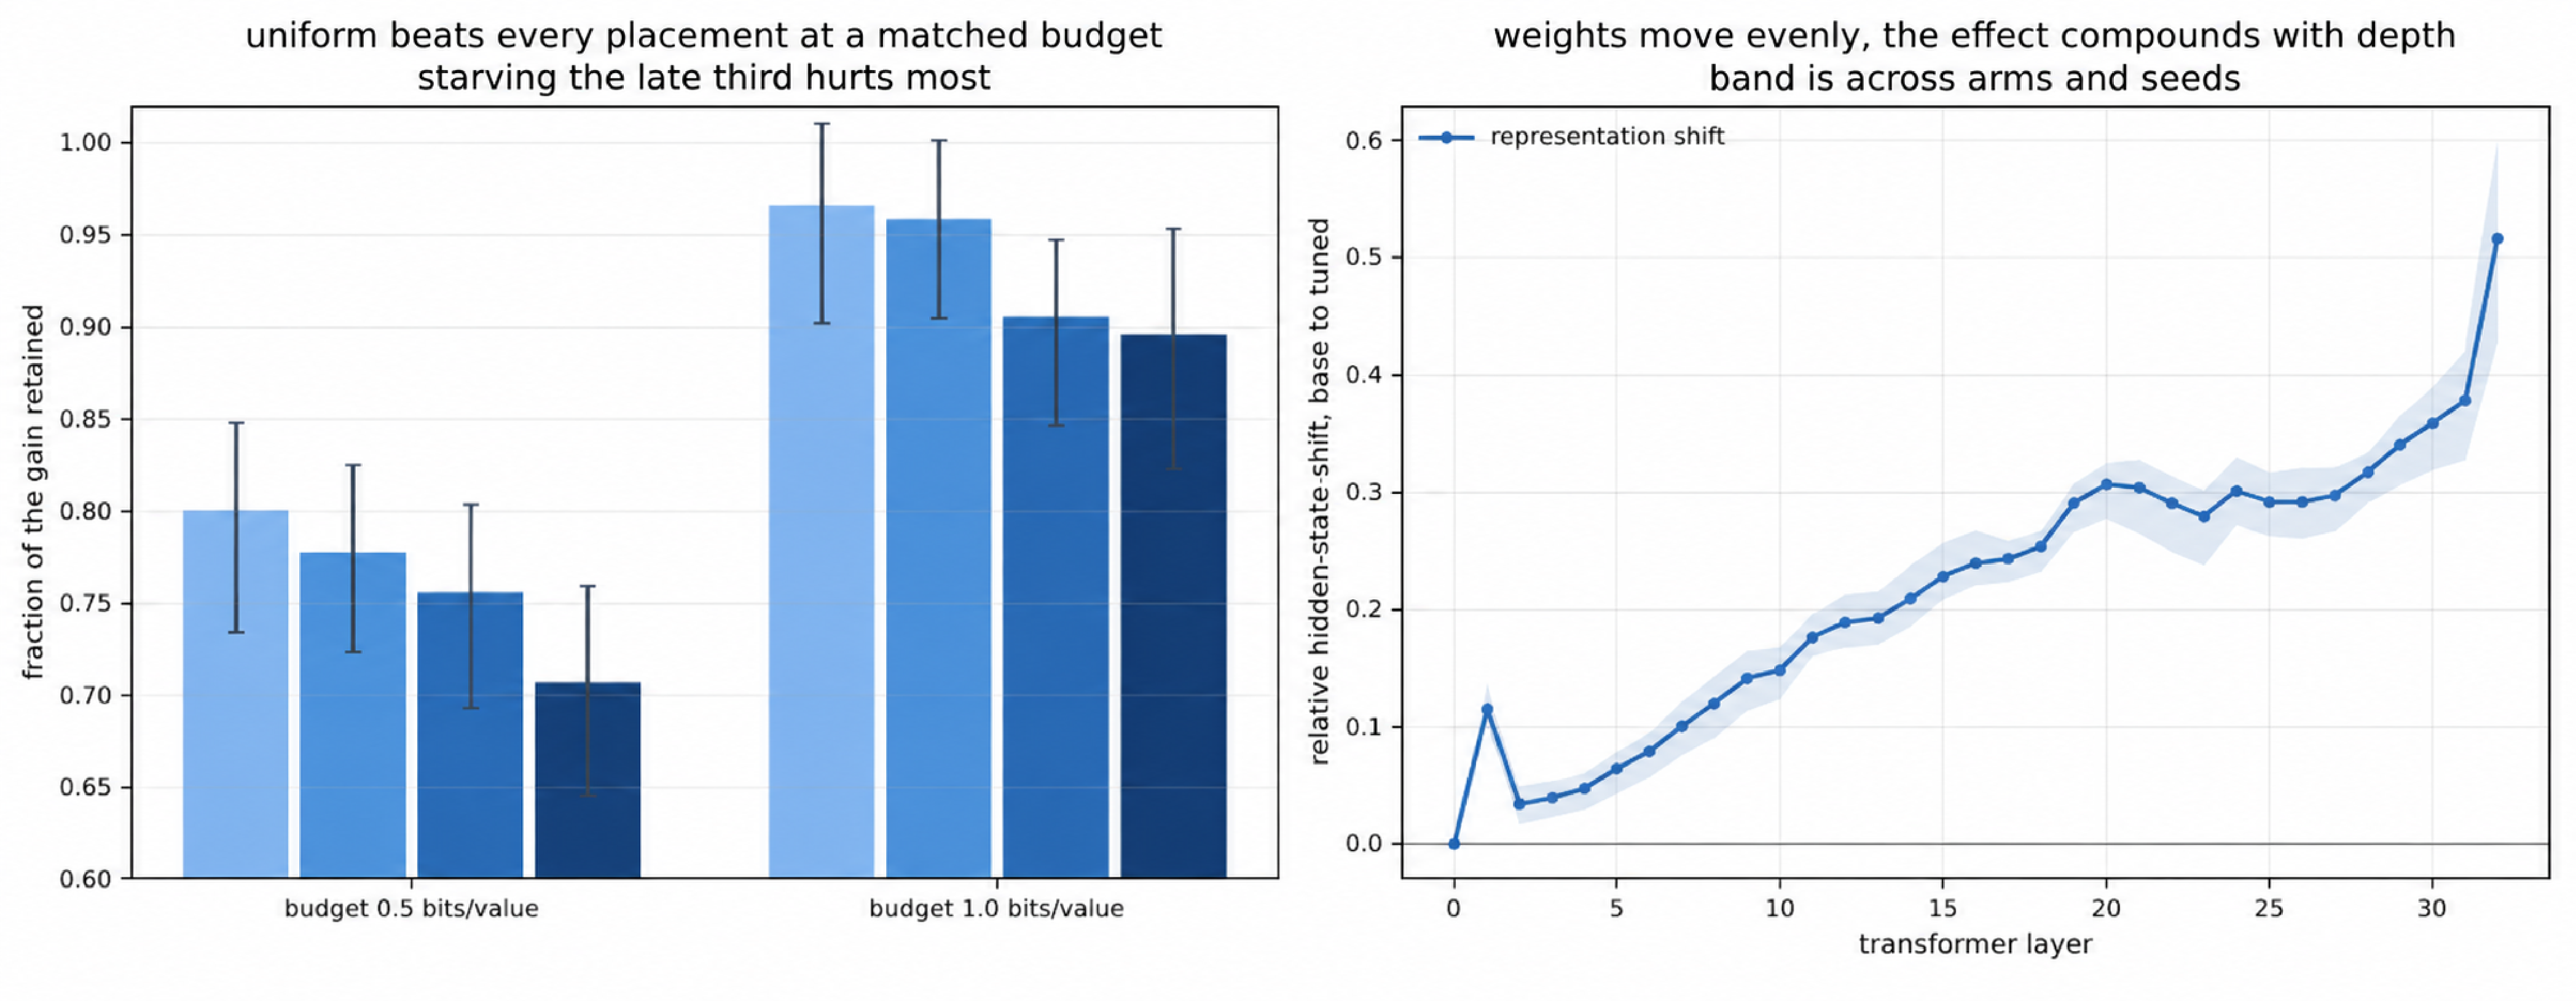
\includegraphics[width=0.8\linewidth]{figures/F4_layer_location.pdf}
\caption{
\textbf{Equal bit budgets are not functionally interchangeable.}
Left: retained gain under uniform or depth-selective compression at matched
budgets. Right: hidden-state shift grows with depth despite approximately
flat update magnitude.
}
\label{fig:layer-location}
\end{figure}

\subsection{The Rate Across Receivers}

\begin{figure}[h]
\centering
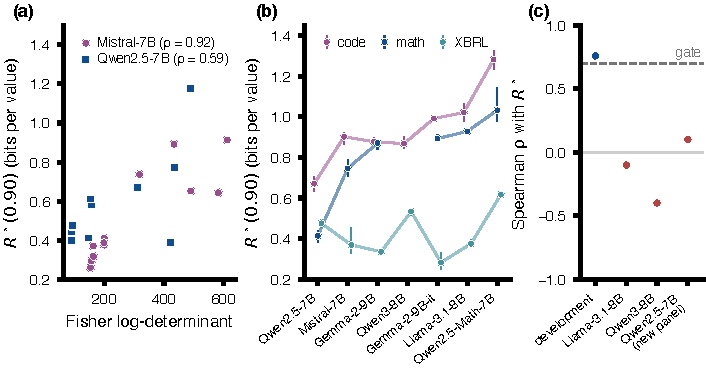
\includegraphics[width=0.8\linewidth]{figures/F10_predictor.pdf}
\caption{The rate belongs to the dataset--receiver pair. (a) Correction-spectrum log-determinant against $R^\star(0.90)$, one point per arm, within the two development receivers. (b) $R^\star(0.90)$ of three corpora on seven receivers; bars span seeds. The ordering of corpora changes with the receiver.}
\label{fig:predictor}
\end{figure}

\subsection{Recovery controls}

\begin{table}[h]
\caption{Accuracy (\%) on GSM8K (1,319) and GSM-Symbolic (500, clustered by template), means of 3 seeds. Frozen base: 77.56 / 71.40. The random rank-1 projection also reaches the base, so direction choice alone does not explain the recovery.}
\label{tab:ladder}
\centering
\small
\begin{tabular}{lrr}
\toprule
condition & GSM8K & GSM-Symbolic \\
\midrule
rank 1 @ 1 bit & \textbf{83.24} & \textbf{77.60} \\
rank 1 @ 16 bits & 42.81 & 33.80 \\
full rank @ 1 bit & 65.05 & 55.00 \\
full rank @ 16 bits (damaged) & 23.81 & 15.53 \\
random rank-1 projection @ 16 bits & 80.09 & 72.13 \\
full update scaled to the rank-1 norm & 23.93 & 13.80 \\
residual rank 15 @ 16 bits & 30.86 & 25.20 \\
\bottomrule
\end{tabular}
\end{table}
% GSM8K 1,319 problems; GSM-Symbolic 500, intervals clustered by template. Qwen2.5-7B, 3 seeds.


\end{document}
